\documentclass[french]{pfia}

% ------------------------------------------
% TITRE
% ------------------------------------------

\title{\textbf{Approche par contraintes pour une classe d'emplois du temps universitaires}}
\usepackage{mathtools}
\usepackage{url}
% please place your own definitions here and don't use \def but
% \newcommand{}{}

%%%%%%%%%%%%%%%%%%%%%%%%%%%%%%%%%%%%%%%%%%%%%%%%%%%%
%% ACRONYMS
\newcommand{\acronym}[1]{{\texttt{#1}}}

\newcommand{\CHR}{\acronym{CHR}}
\newcommand{\C}{\acronym{C}}
\newcommand{\CPP}{\acronym{C++}}
\newcommand{\CSS}{\acronym{CSS}}
\newcommand{\DZN}{\acronym{DZN}}
\newcommand{\FLATZINC}{\acronym{Flatzinc}}
\newcommand{\GECODE}{\acronym{Gecode}}
\newcommand{\JSON}{\acronym{JSON}}
\newcommand{\JAVA}{\acronym{Java}}
\newcommand{\LISP}{\acronym{Lisp}}
\newcommand{\MINIZINC}{\acronym{MiniZinc}}
\newcommand{\PROLOG}{\acronym{Prolog}}
\newcommand{\XML}{\acronym{XML}}
\newcommand{\CHRPP}{\acronym{CHR++}}

\newcommand{\CP}{\acronym{CP}}
\newcommand{\CSP}{\acronym{CSP}}
\newcommand{\DSL}{\acronym{DSL}}
\newcommand{\ITC}{\acronym{ITC}}
\newcommand{\NP}{\acronym{NP}}
\newcommand{\SAT}{\acronym{SAT}}
\newcommand{\UTP}{\acronym{UTP}}


%%%%%%%%%%%%%%%%%%%%%%%%%%%%%%%%%%%%%%%%%%%%%%%%%%%%
%% UTP BUILT-IN TYPES
\newcommand{\SLOT}{H}

\newcommand{\COURSES}{C^{*}}
\newcommand{\COURSE}{C}
\newcommand{\PART}{P}
\newcommand{\CLASS}{K}
\newcommand{\SESSION}{S}

\newcommand{\STUDENT}{U}
\newcommand{\GROUP}{G}
\newcommand{\TEACHER}{T}
\newcommand{\ROOM}{R}

%%%%%%%%%%%%%%%%%%%%%%%%%%%%%%%%%%%%%%%%%%%%%%%%%%%%
%% UTP TYPES
\newcommand{\TYPE}{\mathcal{E}}
\newcommand{\ENTITY}{E}
\newcommand{\EMAP}{F}

\newcommand{\LABEL}{\mathcal{L}}
\newcommand{\RANK}{\mathcal{O}}
\newcommand{\SELECTOR}{\mathcal{F}}

%%%%%%%%%%%%%%%%%%%%%%%%%%%%%%%%%%%%%%%%%%%%%%%%%%%%
%% UTP PROPERTIES
\newcommand{\proptype}[2]{#1^{#2}}
\newcommand{\prop}[3]{\proptype{#1}{#2}_{#3}}

\newcommand{\WEEK}{w}
\newcommand{\WEEKDAY}{d}
\newcommand{\DAILYSLOT}{m}

\newcommand{\PARTALLOWEDSLOT}{d}
\newcommand{\SESSIONDURATION}{length}
\newcommand{\SESSIONRANK}{rank}
\newcommand{\CLASSCAPACITY}{maxsize}
\newcommand{\ROOMCAPACITY}{capacity}
\newcommand{\ROOMDISJUNCTIVE}{disjunct}
\newcommand{\PARTROOMDEMAND}{multi}
\newcommand{\PARTTEACHERDEMAND}{team}
\newcommand{\PARTTEACHERSESSIONS}{service}
\newcommand{\CLASSPARENT}{parents}

\newcommand{\partallowedslots}[1]{\prop{\PARTALLOWEDSLOT}{\SESSION,\SLOT}{#1}}
\newcommand{\sessionduration}[1]{\prop{\SESSIONDURATION}{\SESSION}{#1}}
\newcommand{\rankedsessions}{O}
%\newcommand{\sessionrank}[1]{\prop{\SESSIONRANK}{\SESSION}{#1}}
\newcommand{\classcapacity}[1]{\prop{\CLASSCAPACITY}{\CLASS}{#1}}
\newcommand{\roomcapacity}[1]{\prop{\ROOMCAPACITY}{\ROOM}{#1}}
%\newcommand{\roomdisjunctive}[1]{\prop{\ROOMDISJUNCTIVE}{\ROOM}{#1}}
\newcommand{\disjunctiverooms}{D}%{\ROOMDISJUNCTIVE}
%\newcommand{\oneroom}[1]{\prop{\PARTROOMDEMAND}{\PART}{#1}}
\newcommand{\multiroomparts}{M}%{\PARTROOMDEMAND}
\newcommand{\partteachermultiplicity}[1]{\prop{\PARTTEACHERDEMAND}{\PART}{#1}}
\newcommand{\partteacherservice}[1]{\prop{\PARTTEACHERSESSIONS}{{\TEACHER}\times{\PART}}{#1}}
\newcommand{\classparent}[1]{\prop{\CLASSPARENT}{\CLASS,\CLASS}{#1}}


%%%%%%%%%%%%%%%%%%%%%%%%%%%%%%%%%%%%%%%%%%%%%%%%%%%%
%% UTP MAPS
\newcommand{\maptype}[2]{d^{#1,#2}}
\newcommand{\map}[3]{\maptype{#1}{#2}_{#3}}

%%%%%%%%%%%%%%%%%%%%%%%%%%%%%%%%%%%%%%%%%%%%%%%%%%%%
%% UTP PREDICATES

%{\ADJACENTROOMS}
%{\ATMOSTDAILY}
%{\ATMOSTWEEKLY}
%{\TRAVEL}
%{\FORBIDDENPERIOD}
%{\NOOVERLAP}
%{\SAMEDAILYSLOT}
%{\SAMEDAY}
%{\SAMEROOMS}
%{\SAMESLOT}
%{\SAMESTUDENTS}
%{\SAMETEACHERS}
%{\SAMEWEEKDAY}
%{\SAMEWEEKLYSLOT}
%{\SAMEWEEK}
%{\SEQUENCED}
%{\TEACHERDISTRIBUTION}
%{\WEEKLY}

\newcommand{\ADJACENTROOMS}{adjacent\_rooms}
\newcommand{\ATMOSTDAILY}{at\_most\_daily}
\newcommand{\ATMOSTWEEKLY}{at\_most\_weekly}
\newcommand{\TRAVEL}{travel}
\newcommand{\FORBIDDENPERIOD}{forbidden\_period}
\newcommand{\NOOVERLAP}{no\_overlap}
\newcommand{\SAMEDAILYSLOT}{same\_daily\_slot}
\newcommand{\SAMEDAY}{same\_day}
\newcommand{\SAMEROOMS}{same\_rooms}
\newcommand{\SAMESLOT}{same\_slot}
\newcommand{\SAMESTUDENTS}{same\_students}
\newcommand{\SAMETEACHERS}{same\_teachers}
\newcommand{\SAMEWEEKDAY}{same\_weekday}
\newcommand{\SAMEWEEKLYSLOT}{same\_weekly\_slot}
\newcommand{\SAMEWEEK}{same\_week}
\newcommand{\SEQUENCED}{sequenced}
\newcommand{\TEACHERDISTRIBUTION}{teacher\_distribution}
\newcommand{\WEEKLY}{weekly}
%\newcommand{\NOOVERLAP}{no-overlap}

%allocation\_group
%assign
%domain\_class\_group
%domain\_class\_room
%domain\_session\_teacher
%part\_schedule



%%%%%%%%%%%%%%%%%%%%%%%%%%%%%%%%%%%%%%%%%%%%%%%%%%%%
%% CP VARIABLES
\newcommand{\vartype}[2]{x^{#1,#2}}
\newcommand{\var}[3]{\vartype{#1}{#2}_{#3}}

%% AUXILIARY VARIABLES
\newcommand{\CLASSSIZE}{size}
\newcommand{\ROOMUSE}{use}
%\newcommand{\SESSIONEND}{end}

\newcommand{\classsize}[1]{\prop{\CLASSSIZE}{}{}(#1)}%{\CLASS}{#1}}
\newcommand{\roomuse}[4]{y_{#1,#2,#3,#4}}
%\newcommand{\roomuse}[4]{\prop{\ROOMUSE}{}{}(#1,#2,#3,#4)}
%\newcommand{\sessionend}[1]{\prop{\SESSIONEND}{}{}(#1)}%{\SESSION,\SLOT}{#1}}

%% AUXILIARY VARIABLES REIFYING CONSTRAINTS
\newcommand{\DISJOINT}{split}
\newcommand{\disjoint}[2]{\prop{\DISJOINT}{}{}(#1,#2)}%{\SESSION\times\SESSION}{#1#2}}
\newcommand{\disjointroom}[3]{\prop{\DISJOINT}{}{}(#1,#2,#3)}%{\SESSION\times\SESSION}{#1#2}}


%%%%%%%%%%%%%%%%%%%%%%%%%%%%%%%%%%%%%%%%%%%%%%%%%%%%
%% Maths
\newcommand{\BOOLEAN}{\mathbb{B}}
\newcommand{\NATURAL}{\mathbb{N}}
\newcommand{\myset}[1]{\{#1\}}
\newcommand{\mycard}[1]{|#1|}
\newcommand{\setunion}[3]{\cup_{#1 \in #2}#3}
\newcommand{\setintersection}[3]{\cap_{#1 \in #2}#3}
\newcommand{\setpartition}[3]{\sqcup_{#1 \in #2}#3}
\newcommand{\denote}[1]{\llbracket #1\rrbracket}

%%%%%%%%%%%%%%%%%%%%%%%%%%%%%%%%%%%%%%%%%%%%%%%%%%%%
%% Minizinc syntaxe

% \newcommand{\forallmzn}{\text{forall }}
% \newcommand{\arrowmzn}{\text{->}}
% \newcommand{\inmzn}{\text{ in }}
% \newcommand{\wmzn}{\text{ where }}
% \newcommand{\arraymzn}[1]{\text{#1}}
% \newcommand{\funcmzn}[1]{\text{#1}}
% \newcommand{\gconst}[1]{\text{#1}}
% \newcommand{\const}{\text{constraint  }}
% \newcommand{\subsetmzn}{\text{ subset }}
% \newcommand{\summzn}{\text{sum }}
% \newcommand{\divmzn}{\text{ div }}
% \newcommand{\modmzn}{\text{mod }}
% \newcommand{\intermzn}{\text{ intersect }}
% \newcommand{\equimzn}{\text{<=>}}
% \newcommand{\leqmzn}{\text{>=}}
% \newcommand{\geqmzn}{\text{<=}}

%% Minizinc
\newcommand{\forallmzn}{\text{forall}}
\newcommand{\arrowmzn}{\texttt{ -> }}
\newcommand{\inmzn}{\text{ in }}
\newcommand{\wmzn}{\text{ where }}
\newcommand{\arraymzn}[1]{\text{#1}}
\newcommand{\funcmzn}[1]{\text{#1}}
\newcommand{\gconst}[1]{\text{#1}}
\newcommand{\const}{\text{constraint  }}
\newcommand{\subsetmzn}{\text{ subset }}
\newcommand{\summzn}{\text{sum}}
\newcommand{\divmzn}{\text{ div }}
\newcommand{\modmzn}{\text{ mod }}
\newcommand{\intermzn}{\text{ intersect }}
\newcommand{\equimzn}{\text{<=>}}
\newcommand{\leqmzn}{\texttt{>=}}
\newcommand{\gqmzn}{\texttt{<}}
\newcommand{\lqmzn}{\texttt{>}}
\newcommand{\geqmzn}{\texttt{<=}}
\newcommand{\neqmzn}{\texttt{!=}}
\newcommand{\landmzn}{\text{ /\textbackslash \, }}
\newcommand{\lormzn}{\text{ \textbackslash /}}
\newcommand{\existmzn}{\text{exists}}
\newcommand{\notmzn}{\text{not}}


%% Minizinc 


\newcommand{\xgroup}{\text{x\_groups}}
\newcommand{\xstudent}{\text{x\_group}}
\newcommand{\xroom}{\text{x\_rooms}}
\newcommand{\xteacher}{\text{x\_lecturers}}
\newcommand{\xslot}{\text{x\_slot}}

%% CHR syntax
\newcommand{\xslotstart}{\text{x\_slot\_start}}
\newcommand{\xslotend}{\text{x\_slot\_end}}
\newcommand{\arraychr}[1]{\text{#1}}
\newcommand{\funcchr}[1]{\text{#1}}
\newcommand{\ctchr}[1]{\texttt{#1}}
\newcommand{\chrprop}{\Rightarrow}
\newcommand{\chrsimpl}{\Leftrightarrow}

\usepackage{graphicx}
\usepackage{tabularx}
\usepackage{multirow} 
\usepackage{array}
\usepackage{mathtools}
\usepackage{amsmath}
\usepackage{amssymb}% for disjoint-union operator
\usepackage{stmaryrd}%for denotational brackets
\usepackage{nccmath}
\setlength{\marginparwidth}{2cm}
\usepackage{todonotes}

\newcommand{\davidg}[1]{\todo[inline,color=orange!40]{#1}}
\newcommand{\davidl}[1]{\todo[inline,color=yellow!40]{#1}}
\newcommand{\vincent}[1]{\todo[inline,color=blue!40]{#1}}
\newcommand{\marc}[1]{\todo[inline,color=green!40]{#1}}
\newcommand{\corentin}[1]{\todo[inline,color=pink]{#1}}


% *******************************************************
% **** Listing 
% *******************************************************
% Solarized colors
\definecolor{sbase03}{HTML}{002B36}
\definecolor{sbase02}{HTML}{073642}
\definecolor{sbase01}{HTML}{586E75}
\definecolor{sbase00}{HTML}{657B83}
\definecolor{sbase0}{HTML}{839496}
\definecolor{sbase1}{HTML}{93A1A1}
\definecolor{sbase2}{HTML}{EEE8D5}
\definecolor{sbase3}{HTML}{FDF6E3}
\definecolor{syellow}{HTML}{B58900}
\definecolor{sorange}{HTML}{CB4B16}
\definecolor{sred}{HTML}{DC322F}
\definecolor{smagenta}{HTML}{D33682}
\definecolor{sviolet}{HTML}{6C71C4}
\definecolor{sblue}{HTML}{268BD2}
\definecolor{scyan}{HTML}{2AA198}
\definecolor{sgreen}{HTML}{859900}

\usepackage{listings}
\lstdefinestyle{custom}{
	aboveskip=0.5em,
	belowskip=0em,
	basewidth=0.5em,
	lineskip=-3pt,
	breaklines=true,
	xleftmargin=\parindent,
	showstringspaces=false,
	basicstyle=\small\ttfamily,
%	keywordstyle=\color{sorange},
%	commentstyle=\color{sbase1},
%	stringstyle=\color{sblue},
%	numberstyle=\color{sviolet},
%	identifierstyle=\color{sbase00},
	tabsize=2,
	inputencoding=utf8,
	extendedchars=true,
	literate={Ç}{{\,C}}1 {è}{{\`a}}1 {è}{{\`e}}1 {é}{{\'e}}1,
	escapechar=µ
}

% ------------------------------------------
% AUTEUR(S)
% ------------------------------------------

% 1 auteur
% \author{L. Auteur \\
%  Organisme de rattachement, acronyme laboratoire}
% \date{mél}
 
% plusieurs auteurs 
\author{Vincent Barichard, Corentin Behuet, David Genest, Marc Legeay, David Lesaint\\[6pt]
%\fup{1} Organisme de rattachement 1, acronyme laboratoire 1\\
\fup{1} Univ Angers, LERIA, F-49000 Angers, France \\
%\fup{2} Organisme de rattachement 2, acronyme laboratoire 2\\
%\fup{3} Organisme de rattachement 3, acronyme laboratoire 3\\
}

\date{
\{prenom.nom\}@univ-angers.fr
}

\begin{document}

\maketitle

% ------------------------------------------
% RÉSUMÉS ET MOTS-CLÉS
% ------------------------------------------

\begin{resume}
%\davidl{FAIT : à propager sur EasyChair}
Le calcul d'emplois du temps universitaire est un problème d'optimisation combinatoire complexe tant dans sa modélisation que sa résolution.
Nous proposons une approche par contraintes qui englobe la constitution de groupes, la distribution des salles et enseignants, leur allocation et l'ordonnancement des séances.
Cette approche se fonde sur un langage dédié à base de règles ({\UTP}) 
permettant de modéliser les différentes entités et contraintes d'une instance.
Les instances \UTP{} sont encodées en \XML{} et un générateur convertit les règles en contraintes dans un format %\JSON{} 
compatible avec les solveurs \MINIZINC{} et \CHRPP{}.
Nous présentons dans cet article le langage {\UTP} et ces modèles de programmation par contraintes ainsi que des expérimentations préliminaires réalisées sur un cas d'études concret.
%des instances réelles issues du système universitaire francais.
%
%La résolution repose quant à elle sur un modèle générique développé en {\MINIZINC} et {\CHR} ainsi qu'un parser qui permet de compiler toute instance {\UTP} dans un langage de programation par contraintes et de la résoudre par un solver de contraintes. Nous présentons quelques expérimentations préliminaires menées sur des instances réelles.
\end{resume}

%\begin{motscles}
%%\davidl{FAIT : à propager sur EasyChair}
%Emploi du temps universitaire $\bullet$ Programmation par contraintes $\bullet$ Ordonnancement
%\end{motscles}

\begin{abstract}
%\davidl{FAIT : à propager sur EasyChair}
University course timetabling are complex combinatorial optimization problems to model and solve.
We propose a constraint-based approach which encompasses student sectioning, room and teacher distribution planning, session scheduling and resource allocation.
Our approach is based on a domain-specific rule-based language {\UTP} to model instance entities and constraints.
{\UTP} instances are encoded in {\XML} and a flattener converts rules into constraints using formats supported by \MINIZINC{} and \CHR{}.
This article presents the {\UTP} language and the two constraint programming models as well as early expriments carried out on a real case study. 
\end{abstract}

%\begin{keywords}
%%\davidl{FAIT : à propager sur EasyChair}
%University Timetabling $\bullet$ Constraint Programming $\bullet$ Resource scheduling
%\end{keywords}

% ------------------------------------------
% CORPS DE L'ARTICLE
% ------------------------------------------

%------------------------------------------------------------
%------------------------------------------------------------
\section{Introduction}
\label{sec:introduction}

Course and exam organization in universities involves strategic, tactical and operational decisions relating to curriculum design, student sectioning, course staffing, room planning, class scheduling and resource allocation \cite{2019_lindahl_EJOR}. 
These computational tasks and their overall coordination vary between countries and educational institutions as does the level of process automation and decision tool support \cite{2019_oude_AOR}. 
In French universities for instance  (see Figure~\ref{fig:utp-workflow}), curricula are conventionally revisited every 5 years and students enroll in courses prior to each teaching period in the course of the academic year. Demand is matched by sectioning courses into classes, partitioning students into fixed groups, and populating classes with groups. Eligible groups, lecturers, rooms and equipment are then identified for each course before class sessions get scheduled and allocated the necessary resources. 
Each stage involves different stakeholders with their own requirements (faculty departments, administrative units, course owners, lecturers, tutors, etc.) and the workflow naturally allows for deviations and contingencies (marginal amendments to curricula on a yearly basis, late student registrations, staff absences, etc.).

\begin{figure}[h]
\begin{center}
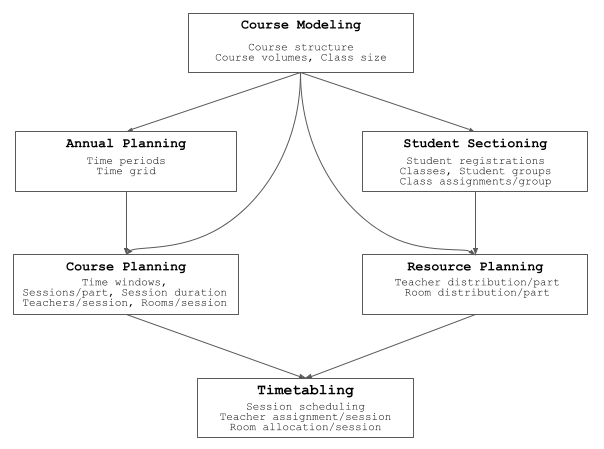
\includegraphics[scale=0.4]{img/utp_workflow.png}
\end{center}
\caption{Conventional workflow for course organization in French universities.}%: steps and roles}
\label{fig:utp-workflow}
\end{figure}

%The scope of these computational tasks and the overall workflow vary between countries and educational institutions as does the level of process automation and decision tool support \cite{2019oudevrielinkAOR}. 
Various problem formulations together with data formats and algorithms 
have been proposed in the literature to tackle specific aspects of university timetabling including 
curriculum balancing %for assigning courses to teaching termes while balancing student workload 
\cite{2001_castro_ARXIV,2012_chiarandini_JH,2013_rubio_MPE}, 
student sectioning \cite{2010_muller_AOR,2019_schindl_AOR}, 
%(strategic) room planning {2017lindhalEJOR}, 
examination timetabling \cite{1996_carter_JORS,2020_battistutta_CPAIOR,2010_mccollum_INFORMS},
curriculum-based %course timetabling \cite{2010mccollumINFORMS,2015bettinelliTOP},
or post-enrolment-based course timetabling \cite{2010_mccollum_INFORMS,2015_bettinelli_TOP,2007_lewis_ITC,2012_cambazard_AOR,2017_goh_EJOR,2021_chen_IEEEA},
tutor allocation \cite{2022_caselli_ESWA},
and minimal timetabling perturbation \cite{2019_lindahl_EJOR,2020_lemos_JS}.
Modeling languages have also been developed, notably the {\XML} language used in the 2019 international timetabling competition \cite{2018_muller_PATAT,2019_ITC} (which we refer to as the {\ITC} language)
which provides a catalog of constraints and supports model variability.
%We adopt a similar approach in this paper and introduce a domain-specific language ({\DSL}) modeling a broad class of university timetabling problems ({\UTP}). %that reduce to hard constraint satisfaction problems ({\CSP}). 
We adopt a similar approach in this paper and introduce a class of university timetabling problems called \UTP{} that involve course scheduling, resource allocation and student sectioning.
%We present a domain-specific language implemented in XML, called \XUTP{}, to encode \UTP{} instances.
%The {\UTP} language provides different features to tailor problem instances to each particular environment. It is designed around a formal domain model and a predicate language to state rules. Each instance is decomposed into a model of entities, a rule set and a solution component. Rules express collections of timetabling constraints on model entities and the solution component lists assignment decisions. Note that the solution may be void, partial or inconsistent. 
We present a domain-specific language to model \UTP{} instances (\UTP{} language) which %provides different features to tailor problem instances to each particular environment. It 
is designed around a formal domain model and a rules language to state constraints. Each instance is decomposed into a model of entities, a rule set and a solution component. Rules express collections of timetabling constraints on model entities and the solution component lists assignment decisions. The latter may be void, partial or inconsistent to accommodate different contexts (e.g., a solution for student sectioning to turn into a complete timetable, an outdated solution that must be revised or repaired). 

%Similarly to the schema proposed in \cite{2018muller,ITC2019} for the international timetabling competition ({\ITC}), 
Similarly to the {\ITC} language, 
the {\UTP} language adopts a multi-scale schedule horizon (i.e., weeks, weekdays and daily slots), a mixed set of resources (i.e., students, student groups, rooms and lecturers), and a hierarchical course structure (i.e., course parts, part classes and class sessions). In our approach however, class sessions (a.k.a., class meetings) are considered as first-class objects that must be scheduled individually alongside resources. 
The model supports single-resource sessions (e.g., single lecturer) as well as multi-resource sessions (e.g., hybrid teaching), and encodes core constraints relating to student sectioning, session scheduling and resource allocation. %which are cast using built-in properties and relations over entities (i.e., resources and course elements) and sessions. 
All resources are assumed cumulative (i.e., rooms, lecturers and students may host, teach and attend overlapping sessions) but this policy may be overridden with disjunctive scheduling rules.
The rules language effectively allows to enforce additional constraints on selected sets of sessions and entities (i.e., resources and course elements).
Rules are expressed using a catalog of timetabling predicates and a comprehension syntax to group, filter and bind sessions and entities. 
Specifically, each rule denotes a conjunction of \UTP{} constraints sharing the same predicate (e.g., periodicity of all lecture classes of a course) and constraints are technically generated through a rule flattening process. %on selected classes of entities and sessions 

%Specifically, the sessions of a course part are cast as single-resource (e.g., face-to-face lectures) or multi-resource sessions (e.g., hybrid sessions) by quantifying the needed resources. 
%Lecturers and rooms are distributed over course parts while students are distributed over courses based on registrations which determines the resources allowed for each session.
%%The resources allowed for a session follow from the distribution of student registrations over courses and that of lecturers and rooms over course parts. 
%The volume of sessions per student depends on individual course registrations as class attendance is compulsory; it is configurable per lecturer in each course part but is unconstrained for rooms. 
%%The volumes of sessions are configurable per teacher in each part (i.e., sessions quota) but pre-determined for students (i.e., class attendance is mandatory) and unconstrained for rooms. 
%No limits apply on simultaneous resource usage but for rooms whose hosting capacity must match class size. Any resource may hence be allocated to joint or overlapping sessions  (e.g., lecture and optional tutoring for students) except for rooms hosting multi-room sessions. In any case, rules may be enforced as needed to prevent sessions from overlapping or to make resources fully disjunctive. As for session scheduling, start time grids are configurable in each course part and the model simply requires full session sequencing in each class. Lastly, the model sections students into classes and supports subgroup inclusion constraints between classes. Note that student groups are considered a by-product of student sectioning and as such may only be listed in the solution component. 

%The rules language allows to state additional constraints using a catalog of timetabling predicates. A rule is tied to a predicate and models a conjunction of constraints on selected classes of entities and sessions (e.g., disjunctive scheduling rule for lecturers, temporal constraints on the courses of a curriculum). Each constraint applies to one or more pairs, called e-maps, and may involve parameters based on the predicate signature. An e-map either associates a resource with a subset of its compatible sessions or a course element with a subset of its constitutive sessions. In the first case, the e-map is interpreted as a set of conditional entity-to-session assignments while it is unconditional if it models a course element. Specifically, a constraint is only evaluated on the sessions for which its e-map argument(s) and the considered solution propose the same entity. Each predicate may be applied equally well to any type of e-map and be used to constrain resources (e.g., lecturer unavailability), course elements (e.g., class periodicity) or individual sessions (e.g., session parallelization). %Note that constraints on e-maps modeling sessions of course elements are de facto unconditional. 
%Formally, a rule is defined by a universally quantified formula wherein quantifiers restrict the domains of the e-map variables. A language of selectors is provided to build and filter domains of e-maps based on session ranks, entity identifiers, entity types, or any user-defined class of elements (e.g., team of lecturers, block of rooms). A rule hence denotes the conjunction of constraints obtained by instantiating the predicate over the cross-product of the domains of the e-map variables. 

\begin{figure}
    \centering
    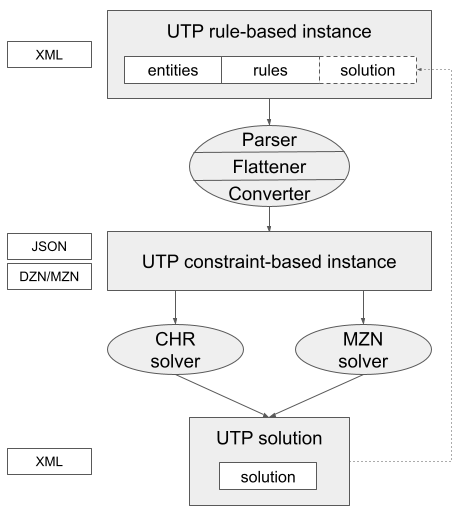
\includegraphics[scale=0.4]{img/utp_toolchain.png}
    \caption{The \UTP{} toolchain.}
    \label{fig:toolchain}
\end{figure}

Note that all constraints are handled as hard constraints and each {\UTP} instance is reduced to a hard constraint satisfaction problem ({\CSP}).
The ability to model preferences and multi-criteria objectives by the means of soft constraints is paramount in course timetabling and will be the subject of future extensions. 
Likewise, the catalog of {\UTP} predicates still lacks important constraints (e.g., gap, distribution and pattern constraints - see e.g. \cite{2017_aizam_AIPCP,2021_chen_IEEEA}) which will be gradually added in future versions.

As for implementation, the \UTP{} language is based on \XML{} and embedded in two constraint modeling languages, namely, 
{\MINIZINC} \cite{2007_nethercote_SPH,MINIZINC} and {\CHR} \cite{1994_fruhwirth_Chap}. 
We developed a tool chain consisting of a \XML{} parser, a rule processor to flatten rules into constraints, and an encoder to convert the resulting instances to solver-compatible formats %using {\JSON} or {\DZN}
(see Figure~\ref{fig:toolchain}). 
Beyond {\MINIZINC} and {\CHR}, constraint-based {\UTP} instances may be used as inputs to any solver implementing the model and predicates of the \UTP{} language.
We do not discuss here the \XML{} syntax of the language (the reader is referred to \cite{uspSite} which provides access to the detailed specification, %the {\JSON/\DZN} instance formats, 
%\cite{uspSite} also provides
the {\MINIZINC} and {\CHR} models, the tool suite, and a benchmark of instances).
Rather, we present the abstract syntax of the \UTP{} language and provide semantics for the key components.

The remainder of the paper is organized as follows.
Section~\ref{sec:schema} introduces the {\UTP} language and draws a comparison with %other modeling frameworks, notably 
the {\ITC} schema.
Section~\ref{sec:model} presents a generic constraint-based {\UTP} model.
Section~\ref{sec:cp-model} discusses its implementation using {\MINIZINC} and {\CHR}
and the cross-validation of the models on a real instance. 
Section~\ref{sec:conclusion} concludes and discusses extensions of this work.
%------------------------------------------------------------
%------------------------------------------------------------
\section{Le langage {\UTP}}
\label{sec:langage-utp}
Le langage {\UTP} décompose la représentation d'une instance 
en 3 composantes : le modèle d'entités, l'ensemble de règles et la solution.
Nous en donnons ici une description informelle. %et
%présentons le catalogue de prédicats,
%le format des règles et des sélecteurs 
%ainsi que leur interprétation sous forme de contraintes. 
Une spécification formelle est présentée dans \cite{uspPATAT22},
et \cite{uspSite}
détaille la syntaxe {\XML} et le format {\JSON} des instances {\UTP}
et donne aussi accès aux codes sources des modèles {\MINIZINC} et {\CHRPP}, aux outils, et à un benchmark d'instances.

%------------------------------------------------------------
%------------------------------------------------------------
\subsection{Modèle d'entités}
\label{sec:entity-model}
Le modèle d'entités d'une instance {\UTP}  est schématisé en Figure~\ref{fig:utp-entity-model}. 
%\corentin{remplacer le schéma de la figure 3 par celui de PATAT => à propager dans APIA aussi}
Il définit l'horizon de temps, la structure
des cours, l'ensemble des ressources, ainsi que des propriétés d'entités et des relations associatives.
L'horizon de temps se décompose en un nombre de semaines, de journées hebdomadaires et de créneaux quotidiens qui sont propres à chaque instance.
%Les semaines partagent les mêmes jours et les jours les mêmes créneaux.
La décomposition des semaines en journées et celle des journées en créneaux quotidiens sont uniformes.
Les semaines et jours se succédant sur l'horizon de temps ne sont pas supposés consécutifs alors que les créneaux quotidiens le sont.
Ces derniers sont de durée égale et divisent la journée de 24h, p. ex., %si la journée se divise en 24 créneaux, ils seront d'une heure chacun. %; 
si elle se divise en 1440 créneaux, 
ils seront d'1 minute chacun.
Les créneaux servent d'unité de temps pour dater démarrage et fin de séances et pour mesurer durées de séance, temps de déplacement entre salles et délais entre séances.

% % For one-column wide figures use
% \begin{figure}[h]
% % \includegraphics{utp-time-grid.eps}
% \caption{{\UTP} 3-layered time grid}
% \label{fig:utp-time-grid}
% \end{figure}

% For one-column wide figures use
\begin{figure*}[ht]
\centering
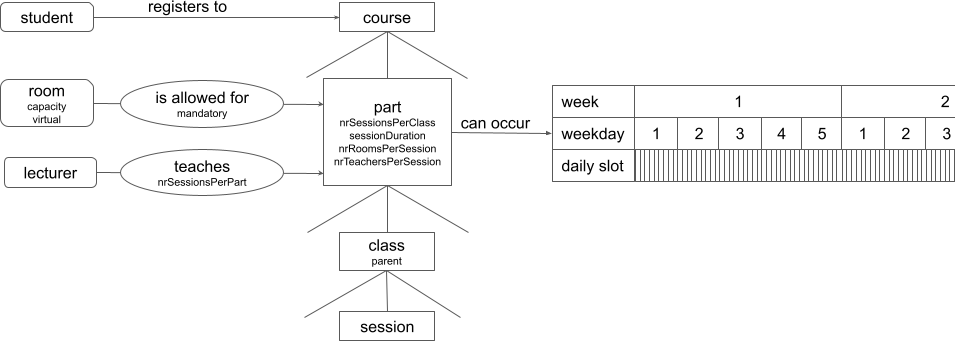
\includegraphics[width=.85\textwidth]{img/utp_entity_model.png}
\caption{Modèle d'entités}
\label{fig:utp-entity-model}
\end{figure*}

Les cours ont une structure arborescente, chaque cours (p. ex. Algo) se décomposant en parties de cours (p. ex. TP d'Algo), chaque partie de cours en classes (p. ex. Classe 2 de TP d'Algo) et chaque classe en séances pré-ordonnées (p. ex. 3\up{ème} séance de la Classe 2 de TP d'Algo).
Les séances sont les tâches élémentaires à ordonnancer quand on résoud une instance {\UTP}, leur nombre, durée et séquencement intra-classe étant fixés.
%Although this approach forbids variable class decompositions, 
%it provides flexibility for handling sessions independently wrt. scheduling and resource allocation.
Précisément, les classes d'une partie de cours comportent un nombre identique de séances de même durée, ces deux constantes étant propres à chaque partie de cours.
%
%Fixed decompositions also facilitates the formulation of requirements which can rely on clear-cut sessions (e.g., planning parallel sessions mid-way through a course, alternating sequences of lecture and practical work sessions).
%
%Les décompositions de manière fixe permettent de faciliter les formulations%TODO
%des besoins%TODO
%en s'appuyant sur un découpages claire des sessions (e.g., planification en parallèle des sessions en milieu de période, faire une alternance entre cours magistraux et travaux pratiques). 
%
%Second, sessions are considered uninterruptible and, in particular, may not overlap two days. 
%Lastly, the schema requires that the sessions of a class be ranked in the entity model and sequenced accordingly in any solution.
D'autre part, le langage impose que les séances d'une classe soient séquencées dans toute solution selon le rang qui leur est associé dans la classe.
Enfin, les séances sont non-interruptibles et en particulier, ne peuvent pas être à cheval sur deux journées.

% % For one-column wide figures use
% \begin{figure}[h]
% % \includegraphics{utp-course-structure.eps}
% \caption{{\UTP} course structure}
% \label{fig:utp-course-structure}
% \end{figure}

%Les ressources{\UTP} fall into 4 types, namely, rooms, teachers, students and (student) groups.
%All the resources of an instance, except groups (see Section~\ref{sec:solutions}), are declared and typed in the entity model.

Trois types de ressources sont modélisés : les salles, les enseignants et les étudiants (constitués en groupes).
Toutes les ressources d'une instance sont déclarées et typées dans le modèle d'entités.
%
%In practice, various restrictions resulting from upstream processes apply on the resourcing and timing of courses (e.g., faculties prescribing degree-specific time grids, departments implementing room pooling policies, alternative candidates designated for teaching courses, students registering for courses).
%
Dans la pratique, différentes contraintes émises en amont s'appliquent aux ressources et aux créneaux de cours (p. ex., facultés imposant une grille horaire par type de cursus, départements mettant en œuvre des politiques de mise en commun de salles, étudiants s'inscrivant aux cours).
%
%Basic restrictions come in the form of compatibility constraints that list the suitable rooms, eligible teachers, candidate students and allowed times for the different courses.
%Such constraints are built in the entity model but scoped differently depending on resource types.
%
Les contraintes les plus élémentaires sont des contraintes de compatibilité énumèrant %liste
les salles appropriées, les enseignants éligibles, les étudiants candidats et les horaires autorisés pour les différents cours.
%
%Precisely, each course part is assigned sets of possible start times, rooms and teachers that are enforced on all its sessions.
Précisément, à chaque partie de cours est assigné l'ensemble des créneaux de départ, de salles et d'enseignants qui sont autorisés pour toutes les séances de la partie (cf. Figure~\ref{fig:utp-entity-model}).
%
%As for students, course registrations are listed separately and %the possible students for a session are those registered to the course it sits in.
%any student registered to a course is considered a possible candidate for each of its sessions.
%Pour les étudiants, l'inscription en cours se fait via une liste qui répertorie tous les cours séparément et tous les étudiants inscrits à un cours sont considéré comme candidat éligible pour chacune de ses sessions.
Concernant les étudiants, l'inscription se fait au niveau des cours, un étudiant devant participer à toutes les parties d'un cours.
La constitution des groupes d'étudiants s'effectue à la résolution du problème ou peut être fournie dans la composante solution. % décrite plus bas.

%Beyond plain compatibility constraints, resource utilization is also subject to demand and capacity constraints.

%Au-delà des simples contraintes de compatibilité, 
L'utilisation des ressources est également soumise à des contraintes de demande et de capacité.
%
%
%Since modalities differ from one environment to the next, the schema supports both disjunctive and cumulative resources as well single- and multi-resource course sessions. 
Comme les modalités diffèrent d'un environnement à un autre, le langage prend en charge les ressources disjonctives et cumulatives ainsi que les séances à ressources uniques ou multiples. 
%
%Students, groups, teachers or rooms qualify as cumulative resources if they 
%can attend, teach or host simultaneous sessions. %, respectively.
Étudiants, enseignants et salles sont qualifiés de ressource cumulative s'ils peuvent suivre, enseigner ou héberger des séances en parallèle.
%
%Cumulative resources are paramount to address flexible attendance requirements (e.g., students assigned optional tutoring sessions that may overlap with mandatory courses) or to handle multi-class events (e.g., rooms hosting joint exam or conference sessions).
Les ressources cumulatives sont indispensables à la modélisation de cours non-obligatoires (p. ex. séances de tutorat facultatives pouvant chevaucher des cours obligatoires) et pour gérer des événements multi-classes (p. ex. salles hébergeant des examens mutualisés).
%
%The schema assumes no limit on the number of parallel sessions teachers and students may attend.
%Rooms however may only host class sessions whose cumulated headcount
%is within their capacity.
Le langage n'impose aucune limite sur le nombre de séances simultanées auxquelles participent enseignants et étudiants.
À l'inverse, les salles ne peuvent héberger que des séances dont l'effectif cumulé est en deça de leur capacité.
%
%Upper bounds on room capacity and class headcounts are encoded for all rooms and classes in the entity model with the possibility to leave room capacity unbounded (e.g., virtual rooms). 
%Note that all resources default to cumulative resources in an entity model and disjunctive behaviour has to be explicitly enforced through rules.
La capacité des salles et les seuils d'effectif des classes sont encodés dans le modèle d'entités qui autorise par ailleurs des salles à capacité illimitée (p. ex. salles virtuelles).
%
Notons que toute ressource est supposée cumulative par défaut
mais des règles disjonctives peuvent être imposées par ressource ou par classe de ressources.
%
%Sessions qualify as multi-resources if they can be allocated multiple resources of the same type at any point in time.

Les séances sont dites multi-ressources si on peut leur allouer plusieurs ressources du même type.
%
%The need for sessions requiring multiple rooms or teachers arises in many practical situations (e.g., multi-room sessions for hybrid teaching, joint supervision of practical work sessions, exams requiring several adjudicators).
Ce type de séances présente un intérêt pratique (p. ex. séances multi-salles pour enseignement hybride, 
séances de travaux pratiques supervisées par plusieurs enseignants, 
examens nécessitant plusieurs surveillants)
et des contraintes s'appliquent alors aux volumes de ressources requis par séance.
Ces dernières s'expriment dans le modèle par des contraintes de cardinalité déclarées sur les parties de cours, chaque partie indiquant le nombre d'enseignants requis par séance (potentiellement aucun) et s'il s'agit de séances à salle unique ou non (\texttt{nrRoomsPerSession} et \texttt{nrTeachersPerSession} en Figure~\ref{fig:utp-entity-model}).
À noter qu'une instance peut mixer des séances
mono-ressource %avec des resoources uniques  
et multi-ressources
et des ressources disjonctives et cumulatives.

Le modèle d'entités incorpore également des contraintes de flot qui
régissent %controle
la distribution des étudiants et des enseignants sur les cours.
Ces contraintes 
sont habituellement émises en amont de la génération d'emplois du temps
durant les phases d'inscription %TODO
et 
de planification de capacité %TODO
(p. ex. distribution des volumes horaires entre enseignants d'un département).
Comme mentionné précédemment, les étudiants s'inscrivent uniquement aux cours. %et non pas aux parties, classes ou séances de cours. 
Résoudre une instance {\UTP} implique donc de placer les étudiants dans les classes conformément à la structure des cours et aux inscriptions demandées.
%
%The implicit rule endorsed in the schema is that a student should be assigned a single class in each part of a course he has registered to and attend all sessions of the selected classes.
La règle adoptée est qu'un étudiant soit assigné à toutes les séances d'une seule classe dans chaque partie de cours.
%
%Group nesting constraints may also be explicitly encoded between classes to enforce equality or set inclusion relations between their sets of participants.
Des contraintes d'imbrication de groupes
peuvent être posées entre classes 
(p. ex. aggréger des groupes de travaux pratiques pour constituer un groupe de cours magistral, préserver les mêmes groupes entre différents cours d'un cursus).
%
%As for staff planning, each teacher is assigned a fixed volume of sessions in each course part it is eligible for, leaving teacher-to-session assignment decisions to solvers.
Pour l'emploi du temps du personnel, chaque enseignant a un volume fixe de séances dans les parties de cours où il intervient, l'affectation des séances restant à déterminer par le solveur.
%
%In addition to built-in types, the schema provides the ability to freely label entities in order to create custom types. 
En complément des types d'entités prédéfinis, le langage offre %permet
la possibilité d'étiqueter
librement les entités du modèle. % afin de créer des types particuliers%personaliser
%
%Precisely, entities sharing the same label in the entity model form a type of their own named after the label.
Les entités qui partagent la même étiquette forment un type à part entière. % nommé d'après cette étiquette.
%
%Labels complement the built-in types and both are used as a means to select entities within rules.
Ces étiquettes peuvent être utilisées à l'instar des types prédéfinis pour sélectionner les entités dans les règles.

%------------------------------------------------------------
%------------------------------------------------------------
\subsection{Ensemble de règles}

\begin{table*}[ht]
%\resizebox{\textwidth}{!}{%
\small
\centering
\begin{tabular}{|l|l|l|p{.6\textwidth}|}
\hline
\textbf{Nom}               & \textbf{Arité} & \textbf{Paramétrique} & \textbf{Sémantique}\\ \hline

%assign\_slot               & 1         & yes   & Assign a slot or slot tuple to a session\\ \hline
%assign\_room               & 1         & yes   & Assign a set of room to session in entry\\ \hline

%allocation\_group           & 1        & no    & Domain allocation for class with group in the solution\\ \hline
%part\_schedule              & 1        & no    & Allowed start time slots for sessions\\ \hline
%domain\_class\_group        & 1        & no    & Allowed groups for classes (solution input)\\ \hline
%domain\_session\_teacher    & 1        & no    & Allowed teachers for sessions\\ \hline
%domain\_class\_room         & 1        & no    & Allowed rooms for sessions\\ \hline

{\SAMEDAILYSLOT}            & 1         & non    & Les séances démarrent le même créneau quotidien\\ \hline
{\SAMEWEEKDAY}              & 1         & non    & Les séances démarrent la même jour de la semaine\\ \hline
{\SAMEWEEKLYSLOT}           & 1         & non    & Les séances démarrent les mêmes créneau et journée\\ \hline
{\SAMEWEEK}                 & 1         & non    & Les séances démarrent la même semaine\\ \hline
{\SAMEDAY}                  & 1         & non    & Les séances démarrent le même jour\\ \hline
{\SAMESLOT}                 & 1         & non    & Les séances démarrent en même temps\\ \hline
{\FORBIDDENPERIOD}          & 1         & oui   & Les séances ne peuvent pas débuter dans la période donnée\\ \hline
{\ATMOSTDAILY}              & 1         & oui   & Le nombre de séances dans la période journalière définie est limité\\ \hline
{\ATMOSTWEEKLY}             & 1         & oui   & Le nombre de séances dans la période hebdomadaire définie est limité\\ \hline
%implicit\_sequenced\_sessions & 1 & \multicolumn{4}{|c|}{no} & All sessions in classes are sequenced\\ \hline
{\SEQUENCED}                & $\geq2$   & non    & Les séances sont séquencées\\ \hline
{\WEEKLY}                   & 1         & non    & Les séances démarrent les mêmes créneaux et jours de semaines successives \\ \hline

{\NOOVERLAP}                & 1         & non    & Les séances ne peuvent être en parallèle\\ \hline
{\TRAVEL}                   & 1         & oui   & Définition du temps de trajet entre salles\\ \hline

{\SAMEROOMS}                & 1         & non    & Les séances ont lieu dans les mêmes salles\\ \hline
{\SAMESTUDENTS}             & 1         & non    & Les mêmes étudiants suivent les séances\\ \hline
{\SAMETEACHERS}             & 1         & non    & Les séances sont encadrées par les mêmes enseignants\\ \hline

{\ADJACENTROOMS}            & 1         & oui   & Les séances doivent être dans des salles adjacentes\\ \hline

{\TEACHERDISTRIBUTION}      & $\geq2$   & oui   & Distribue la charge des enseignants dans les classes\\ \hline

\end{tabular}
%}
\caption{Catalogue des prédicats {\UTP}}
\label{tab:catalogue_predicats}
\end{table*}

Les règles sont utilisées pour formuler des conjonctions de contraintes.
Il s'agit de pouvoir exprimer, de manière concise, une ou plusieurs contraintes liées à un même prédicat.
L'expression d'une règle implique d'identifier l'ensemble des séances que l'on souhaite contraindre et de choisir le prédicat à appliquer.
La table~\ref{tab:catalogue_predicats} liste les prédicats \UTP{} actuellement implémentés et utilisés dans nos instances.

Une règle porte, selon l'arité de son prédicat, sur un ou plusieurs domaines d'e-maps qui associent chacune une entité à un ensemble de séances compatibles.
Les domaines d'e-maps ne sont pas représentés en extension mais à l'aide de sélecteurs. 
Un sélecteur permet de cibler des entités selon leur type, leur étiquette ou leur identifiant et de filtrer les ensembles de séances associées selon leurs rangs et leur compatibilité avec d'autres entités.
%Un sélecteur permet ainsi de réduire l'ensemble de toutes les séances à un sous-ensemble selon si les séances sont liées à une entité spécifique (un élément de cours comme une partie, ou une ressource comme un enseignant), et en fonction de leur rang (pour sélectionner la $n$-ième séance).
%Un sélecteur combine un générateur et une liste optionnelle de filtres.
%Les filtres et le générateur s'expriment de la même manière, le générateur permettant d'indiquer comment les séances doivent être regroupées.
%L'ensemble des séances d'un sélecteur est l'intersection des ensembles de séances du générateur et éventuellement des filtres.
%L'ensemble des séances de la règle est le produit cartésien des ensembles de séances définis par les sélecteurs.
Une règle se traduit ensuite par la conjonction de contraintes obtenue en instanciant le prédicat sur le produit cartésien des domaines d'e-maps sélectionnées.
%Lorsque le type du générateur ou du filtre est une ressource, alors la contrainte générée par la règle ne s'appliquera qu'aux séances réellement associées à la ressource.
%
%Generators and filters are triples 
%$
%(T_i,L_i,O_i)
%$
%consisting of
%an entity type
%$
%T_i%\in{\TYPE}
%$,
%an entity label or identifier
%$
%L_i%\in{\LABEL}
%$
%and
%a subset of session ranks
%$
%O_i%\subseteq{\RANK}
%$ (a.k.a., session mask),
%the latter two elements being optional.
%A selector 
%matches any e-map
%whose entity satisfies the type, label and identifier constraints of the generator
%and whose %set of sessions 
%image includes any compatible session
%satisfying the mask of the generator
%and one of the filters.
%Note that rules featuring empty selectors are discarded during the flattening stage. 
%%Selectors are encoded as attributes in the {\XML} language
%%using a syntax that borrows from the CSS selector language.
%%For instance, the above example would be encoded by the following XML fragment: 
%%\todo[inline]{Marc : Rajouter une phrase pour décrire brièvement la figure 3}

\begin{figure*}[h]
\centering
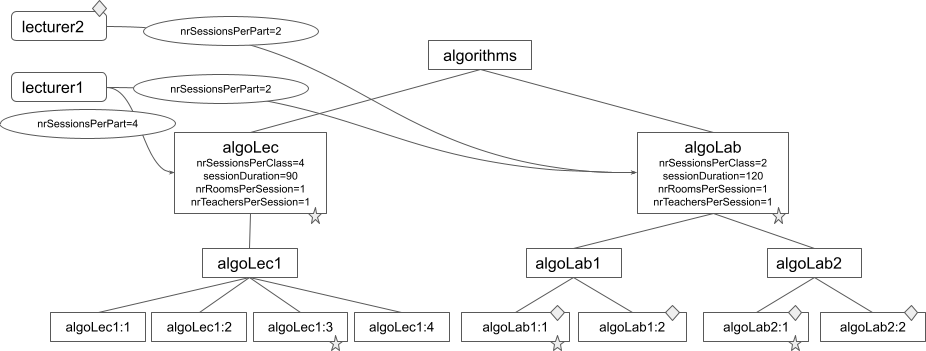
\includegraphics[scale=.45]{img/utp_rule_1.png}

%{\small{
%\begin{flalign}
%&\texttt{{\FORBIDDENPERIOD}((<(\TEACHER,{teacher2},\_)>,9120,9240)}
%&\label{rule-example-1}
%\\
%&\texttt{{\SEQUENCED}(<(\CLASS,\_,\myset{3}),(\PART,{algoLec},\_)>}
%\texttt{\mbox{<(\CLASS,\_,\myset{1}),(\PART,{algoPra},\_)>)}}
%&\label{rule-example-2}
%\end{flalign}
%}}
\newcounter{save_equation}
\setcounter{save_equation}{\value{equation}}
\setcounter{equation}{0}

\renewcommand{\theequation}{R\arabic{equation}}

{\footnotesize{
\begin{flalign}
&\texttt{{\SEQUENCED}(<(\CLASS,\_,\myset{3}),(\PART,{algoLec},\_)>,
<(\CLASS,\_,\myset{1}),(\PART,{algoLab},\_)>)}
&\label{rule-example-1}
\\
&\texttt{{\FORBIDDENPERIOD}((<(\TEACHER,{lecturer2},\_)>,9120,9240)}
&\label{rule-example-2}
\end{flalign}
}}


\setcounter{equation}{0}
\renewcommand{\theequation}{C\arabic{equation}}

%
{
\footnotesize
\begin{flalign}
&\texttt{{\SEQUENCED}((algoLec1,\{algoLec1:3\}), (algoLab1,\{algoLab1:1\}))}
&\label{constraint-example-1}
\\
&\texttt{{\SEQUENCED}((algoLec1,\{algoLec1:3\}), (algoLab2,\{algoLab2:1\})}
&\label{constraint-example-2}
\\
&\texttt{{\FORBIDDENPERIOD}((lecturer2,\{algoLab1:1,algoLab1:2,algoLab2:1,algoLab2:2\}),9120,9240)}
&\label{constraint-example-3}
\end{flalign}
}
%

\caption{Sélection de séances par des règles}
\label{fig:utp-rule-1}
\end{figure*}

%Figure~\ref{fig:utp-rule-1} illustrates the rules flattening process on a small example.
%Course \texttt{algorithmic} is split into a lecture part \texttt{algoLec} and a practice part \texttt{algoPra}.
%The lecture part has a single class of 4 sessions taught by \texttt{teacher1} and the practice part has 2 classes of 2 sessions each taught by \texttt{teacher1} or \texttt{teacher2}.
%%Figure~\ref{fig:utp-rule-1} illustrates the flattening of the following rules: 
%%on a simple model consisting of 2 teachers and & course subdivided into 2 parts, 3 classes and 8 sessions. The first rule forbids a time period for 
%Rule~(\ref{rule-example-1}) below requires that teacher \texttt{teacher2} have no session between $9120$ and $9240$, that is, between 8am and 10am on Tuesday of week 2. 
%%In this rule, $9120$ (resp. $9240$) is the value\footnote{Each possible session schedule is mapped to a single value. All possible values make up the domain of a session.} that corresponds to 8am on Tuesday (resp. 10am on Tuesday) of week 2. 
%The selector includes no mask and no filter hence matches with all possible sessions of \texttt{teacher2} as indicated with diamonds on Figure~\ref{fig:utp-rule-1}. 
%The resulting domain of e-maps is the singleton $\myset{(teacher2,\map{\TEACHER}{\SESSION}{teacher2})}$ and the rule is flattened into a single \texttt{\FORBIDDENPERIOD} constraint. %%$\myset{\map{\TEACHER}{\SESSION}{teacher2}}$.
%Rule~(\ref{rule-example-2})
%%requires that the first practical session in Algorithmic \todo[inline]{Marc : pourquoi algo ?} start after the third lecture.
%requires that the first sessions of the practices start after the third lecture.
%The two selectors include a filter. The first selector matches with all class sessions of rank 3 in part \texttt{algoLec}, and the second matches with all class sessions of rank 1 in part \texttt{algoPra} as indicated with stars on the figure.
%The rule is flattened into 2 \texttt{\SEQUENCED} constraints corresponding to the cross product of the e-map domains $\myset{(algoLec1,\map{\RANK}{\SESSION}{3}\cap\map{\PART}{\SESSION}{algoLec})}$ and $\myset{(algoPra1,\map{\RANK}{\SESSION}{1}\cap\map{\PART}{\SESSION}{algoPra}),(algoPra2,\map{\RANK}{\SESSION}{1}\cap\map{\PART}{\SESSION}{algoPra})}$.


La Figure~\ref{fig:utp-rule-1} illustre la sélection de séances sur un exemple jouet et la génération automatique de contraintes à partir de deux règles.
Le cours \texttt{algorithms} est divisé en une partie de cours magistraux \texttt{algoLec} et une partie de travaux pratiques \texttt{algoLab}.
Le cours magistral est dispensé par \texttt{lecturer1} et ne contient qu'une classe de 4 séances. Les travaux pratiques sont encadrés par \texttt{lecturer1} et \texttt{lecturer2}, et sont constitués de 2 classes de 2 séances.

La première règle (\ref{rule-example-1}) %Deux règles sont illustrées : % en Figure~\ref{fig:utp-rule-1}
stipule que les travaux pratiques de chaque classe ne peuvent commencer qu'après la troisième séance de cours magistral (entités et séances annotées avec une étoile).
Elle est associée au prédicat \texttt{\SEQUENCED} et utilise deux sélecteurs : le premier sélectionne la troisième séance de la partie \texttt{algoLec}, le second sélectionne, pour chaque classe, les premières séances de la partie \texttt{algoLab}.
La partie \texttt{algoLab} ayant deux classes, la règle produit deux contraintes liées à \texttt{\SEQUENCED} : la première (\ref{constraint-example-1}) avec les séances \texttt{algoLec1:3} et \texttt{algoLab1:1}, la seconde (\ref{constraint-example-2}) avec les séances \texttt{algoLec1:3} et \texttt{algoLab2:1}.

La seconde règle (\ref{rule-example-2}) stipule que \texttt{lecturer2} est indisponible sur une période donnée (losanges).
Elle est associée au prédicat \texttt{\FORBIDDENPERIOD} et utilise un sélecteur qui cible les séances de l'enseignant \texttt{lecturer2}.
La règle produit une seule contrainte (\ref{constraint-example-3}) liée à \texttt{\FORBIDDENPERIOD} (avec les paramètres spécifiant la période d'absence de l'enseignant, ici la période entre les créneaux 9120 et 9240) portant sur l'ensemble des séances de la partie \texttt{algoLab} où peut intervenir \texttt{lecturer2}.
La contrainte ne sera effective que sur deux de ces séances étant donné que \texttt{lecturer2} encadre deux séances de travaux pratiques ; ces séances seront identifiées pendant la résolution.




%------------------------------------------------------------
%------------------------------------------------------------
\subsection{Solution}
%The solution component includes assignment decisions relating to the choice of slots and resources for sessions, the placement of students in groups and the assignment of groups to classes.
%The solution hence represented may be partial, see empty, and does not have to be consistent with the built-in constraints or the rules of the instance.
%The support for partial solutions allows to tackle subproblems using separate {\UTP} instances and solution seeds.
%For instance, a scheduling instance may be defined on the basis of partial and consistent solutions pre-generated for the student sectioning and resource allocation subproblems.
%Likewise, the support for inconsistent solutions is paramount to repair solutions that have become inconsistent due to unforeseen changes.
L'élément solution comporte des choix de créneaux et de ressources pour les séances, de groupes pour les étudiants, et de classes pour les groupes.
La solution ainsi représentée peut être partielle, voire vide, et n'est pas nécessairement consistante avec les contraintes de l'instance.
Le support des solutions partielles permet de cibler et résoudre des sous-problèmes. %en utilisant différentes instances \UTP{}.
Par exemple, une instance se réduit à un problème d'ordonnancement si elle se base sur une solution complète pour la constitution des groupes et l'affectation des ressources.
De même, le support des solutions inconsistantes est un pré-requis pour la réparation de solutions qui seraient devenues inconsistantes suite à des changements non-anticipés (p. ex. absence d'un enseignant, indisponibilité d'une salle suite à des travaux).

%%As mentioned before, 
%Student groups are considered a by-product of student sectioning.
%For this reason, groups may only be listed in the solution component, not in the entity model, and defined both by the students they include and the classes they are assigned to. 
%This sectioning process is subject to different constraints. 
%First, groups may only include students with identical course registrations.
%Second, students are inextricably bound to their group, % and indirectly assigned sessions 
%that is, students must be partitioned into groups consistently with their registration profile. %which are given in the entity model.
%Third, group-to-class assignments must comply with any subgroup inclusion constraint stated in the entity model.
Les groupes d'étudiants sont considérés comme le résultat du problème de sectionnement.
Pour cette raison, les groupes font partie de l'élément solution, et définissent à la fois l'ensemble des étudiants qui les composent et les classes auxquelles ils appartiennent.
Ce processus de sectionnement est soumis à différentes contraintes.
D'une part, les groupes ne peuvent être constitués que d'étudiants qui sont inscrits aux mêmes cours.
Ensuite, chaque groupe est insécable sauf dans le cas de séances multi-salles.
Enfin, l'affectation des groupes aux classes doit satisfaire aux contraintes d'inclusion entre classes définies dans le modèle d'entités.









%------------------------------------------------------------
%------------------------------------------------------------
\subsection{Etat de l'art}
\label{2022_JFPC/etat_art}
Nous dressons ici une comparaison du langage {\UTP} et du cadre de représentation {\ITC} implémenté en {\XML} \cite{2018muller,ITC2019}.

Les deux approches se distinguent d'abord par la modélisation des programmes (ordonnancements) possibles par classe.
Le langage {\UTP} définit chaque classe par une simple séquence de séances de durée égale et le problème consiste à programmer chaque séance.
Le schéma {\ITC} %, quant à lui, 
procède en extension et associe différents programmes à chaque classe (élément {\texttt{times}} du schéma).
Le problème se ramène alors au choix d'un programme par classe
où chaque programme est figé et se définit par la répétition sur plusieurs semaines d'un planning hebdomadaire comportant une ou plusieurs séances de durée égale, placées sur différentes journées et partageant le même créneau quotidien.
Les deux représentations ne se réduisent pas l'une à l'autre.
Par exemple, {\UTP} ne peut modéliser une classe dont les séances sont de durées variables.
A l'inverse, {\ITC} ne peut modéliser une classe programmée sur différents créneaux quotidiens.
Toutefois, certains programmes d'intérêt pratique se représentent dans l'une ou l'autre approche en contraignant classes et séances de manière appropriée.
Par exemple, une classe hebdomadaire devant se rencontrer sur le même créneau se modélise en combinant des contraintes \texttt{\SAMEDAILYSLOT}, \texttt{\WEEKLY} et \texttt{\FORBIDDENPERIOD}.
L'implémentation d'une méthode de réduction plus complète %(par exemple, par le biais de prédicats dédiés) 
est en cours d'étude.

Pour ce qui concerne l'organisation hiérarchique des cours, 
{\ITC} introduit un niveau intermédiaire modélisant un choix de configuration par cours (élément {\texttt{configuration}}).
Chaque cours possède une ou plusieurs configurations qui sont indépendantes quant à leur décomposition en parties, classes et séances. 
Le schéma {\ITC} impose simplement qu'un étudiant inscrit à un cours assiste à toutes les parties d'une seule configuration, deux étudiants pouvant être associés à des configurations différentes. %\davidg{On ne dit rien à propos de UTP à ce propos. En ne disant rien, on laisse à penser que ceci ne peut pas être pris en compte dans UTP. Je sais bien qu'on est "serrés" donc pas forcément nécessaire de prendre en compte cette remarque. }
Ce concept n'est pas intégré dans la version actuelle du langage {\UTP}.
Pour ce qui concerne les ressources, le langage {\UTP} représente explicitement les enseignants à l'instar des salles alors qu'{\ITC} ne modélise que les salles.
Il permet aussi d'allouer différentes ressources aux séances d'une même classe 
%(et en particulier de spécifier le service d'enseignement de chaque intervenant)
alors que le schéma {\ITC} impose qu'une même salle leurs soit allouée.
En outre, {\UTP} autorise des séances multi-ressources alors qu'{\ITC} est restreint aux séances mono-salles.

Les deux languages de contraintes %proposés %dans {\UTP} et {\ITC} 
se démarquent aussi l'un de l'autre. 
D'une part, les prédicats {\ITC} s'appliquent aux classes alors que
les prédicats {\UTP} s'appliquent à des ensembles de séances quelconques - et en particulier à des séances individuelles - qui peuvent être conditionnés au choix des ressources allouées. 
D'autre part, le langage de règles et de sélecteurs {\UTP} permet de contraindre n'importe quelle classe de ressources ou d'éléments de cours de manière concise et plus adaptée pour l'expression des besoins.

Enfin, le schéma {\ITC} prescrit une résolution du problème par optimisation combinatoire en intégrant une fonction coût pondérant 4 critères qui pénalisent respectivement les choix de créneaux et de salles pour les classes, les violations de contraintes et le chevauchement de séances par étudiant.
Dans sa version actuelle, le langage {\UTP} traite le problème comme un problème de satisfaction de contraintes dures.
L'intégration de contraintes souples et la possibilité d'aggréger pénalités ou préférences, que ce soit dans des contextes de construction ou de réparation de solution, est à l'étude.

%Student groups 
% near-identical course structure: no course configuration element
% no time elements in UTP classes. Alternative class times are fixed in ITC
% OK time elements in extension -> unusitable for loosely constrained class programs
% OK impossible to express k weekly slots with different starting slots. In UTP: use sameWeeklySlot with masks.
% OK impossible to enforce different constraints bettwen first period of a course (amorcage) and the rest => ok for us with masks
% KO: times with different #sessions and session length. 
% => solution per session (vs per class) : slot + romms + teachers


%Sectioning:: as itc (parent class)
%Ressources
%- rooms: travel in ITC => using constraint travel in UTP.
%- new: teachers.
%- students: no change.
%- OK groups. Admin and computational needs.
%- Domain constraints
%- by default, all resources are cumultative (explain). Avec contrainte (disjunctive):: no overlap on romms/etc. 
%- allowed slot (applies to all sessions of a part's classes) : ITC via time elements. Adequate for "grid systems". 
%- allowed rooms and allowed teachers (worklaod per part = prescribed number of sessions)
%- single or multi-room/teacher session in UTP.
%- possibly different resources between sessions of a class (unless addiiotnal rules:: sameRoom, sameTeacher, ...)
%Rules language
%- ITC: class-level constraints vs session-level constraints on UTP
%- Labelling: simplifies constraint expression to look up entities
%Solution
%seul ajout: group-to-class and student-to-group
%Résolution: UTP == SAT vs Opt/gestion prefs => pas de priorites, pondérations, etc
%

%------------------------------------------------------------
%------------------------------------------------------------
\section{Modèles \MINIZINC{} et \CHR{}}% des instances \UTP}
\label{sec:model}
\setcounter{equation}{0}
Nous présentons dans cette section deux modèles d'instances {\UTP} développés en \MINIZINC{} et \CHR{}.
Ces modèles mettent en jeu des contraintes relatives
au partitionnement des étudiants en groupes et à l'attribution des groupes aux classes,
à la distribution des ressources sur les séances,
à l'ordonnancement des séances,
et à l'allocation de leurs ressources.
%\davidl{Expliquer transformation du modèle UTP en modèle PPC : "manuel" + built-ins:predicates}
Nous présentons tout d'abord les données d'instance
ainsi que les variables de décision qui sont communes aux deux modèles.
%La table~\ref{table:cp-core-sets} liste les plages d'entiers identifiant les différents ensembles d'objets manipulés.
%(p. ex., ensemble des séancesset of compatible sessions for rooms) and metric properties (e.g., room capacity). 
La table~\ref{table:cp-instance-data} liste les plages d'entiers identifiant les différents ensembles d'objets manipulés et définit les structures utilisées pour représenter les données d'instance.


\begin{table}[!ht]
%\resizebox{\textwidth}{!}{%
\centering
\framebox[\columnwidth][c]{%
\small
\begin{tabularx}{\columnwidth}{>{\hsize=0.01\hsize\linewidth=\hsize}X>{\hsize=1.89\hsize\linewidth=\hsize}X>{\raggedleft\arraybackslash\hsize=.09\hsize\linewidth=\hsize}X}
%\small
%\begin{tabularx}{\columnwidth}{|p{.35\columnwidth}p{.55\columnwidth}|}
%\hline
\SLOT & ensemble des créneaux définissant l'horizon de temps \\
%& (1..(nr\_daily\_slot $\times$ nr\_week\_day $\times$ nr\_week))\\ 
\COURSE & ensemble des cours\\
\PART & ensembles des parties de cours\\
\CLASS & ensembles des classes\\
\SESSION & ensembles des séances\\
\ROOM & ensemble des salles\\
\TEACHER & ensemble des enseignants\\
\GROUP & ensemble des groupes d'étudiants\\
\STUDENT & ensembles des étudiants\\
\hline
%class\_groups               & \\
\multicolumn{2}{p{.9\columnwidth}}{class\_\{sessions,parents\} :} \\
& ensemble des séances (resp. classes parentes) d'une classe \\
%class\_sessions             & \\
%group\_students             & \\
\multicolumn{2}{p{.9\columnwidth}}{part\_\{classes,lecturers, rooms,sessions\} :} \\
 & ensemble des classes (resp. enseignants, salles, séances) d'une partie \\
%part\_lecturers             & \\
%part\_rooms                 & \\
%part\_sessions              & \\
\multicolumn{2}{p{.9\columnwidth}}{room\_sessions :}\\
& ensemble des séances possibles pour une salle\\
\multicolumn{2}{p{.9\columnwidth}}{session\_\{part,class\} : la partie (resp. classe) d'une séance} \\
%session\_class              & \\
\multicolumn{2}{p{.9\columnwidth}}{student\_\{courses,parts\} :}\\
 & les cours (resp. parties) que suit un étudiant \\
%student\_parts              & \\

\multicolumn{2}{p{.9\columnwidth}}{mandatory\_rooms : les salles obligatoires pour une partie} \\
\multicolumn{2}{p{.9\columnwidth}}{single\_room\_sessions : l'ensemble des séances mono-salle} \\
\multicolumn{2}{p{.9\columnwidth}}{capacity : capacité maximum d'une salle ou d'une classe} \\
\multicolumn{2}{p{.9\columnwidth}}{is\_multi\_rooms : indique si une séance est multi-salles} \\
\multicolumn{2}{p{.9\columnwidth}}{length : durée d'une séance} \\
\multicolumn{2}{p{.9\columnwidth}}{part\_room\_use :}\\
 & modalité d'utilisation de salles pour une partie (none, single, multiple) \\
\multicolumn{2}{p{.9\columnwidth}}{rank : rang d'une séance} \\
\multicolumn{2}{p{.9\columnwidth}}{service :} \\
 & nombre de séances à dispenser par enseignant par partie \\
\multicolumn{2}{p{.9\columnwidth}}{teams :} \\
 & nombre d'enseignants requis par séance d'une partie \\
\multicolumn{2}{p{.9\columnwidth}}{virtual : indique si une salle est de capacité illimitée ou non} \\
\multicolumn{2}{p{.9\columnwidth}}{dailyslots : créneaux quotidiens autorisés pour une partie} \\
\multicolumn{2}{p{.9\columnwidth}}{weekdays : journées autorisées pour une partie} \\
\multicolumn{2}{p{.9\columnwidth}}{weeks : semaines autorisées pour une partie} \\
\multicolumn{2}{p{.9\columnwidth}}{nr\_daily\_slots : nombre de créneaux dans une journée} \\
\multicolumn{2}{p{.9\columnwidth}}{nr\_weekly\_slots : nombre de créneaux dans une semaine}\\
%part\_*                     & entité, séance ou valeur associée aux partie de cours\\
%class\_*                    & entité, séance ou valeur associée aux classes\\
%%part\_sessions              & séances d'une partie de cours\\
%%class\_sessions             & séances d'une classe\\
%%part\_ressources            & ressources allouables dans une partie de cours\\
%%part\_daily\_slots          & créneaux quotidiens autorisés pour une partie de cours\\
%%part\_weekdays              & journées hebdomadaires autorisées pour une partie de cours\\
%%part\_weeks                 & semaines autorisées pour une partie de cours\\
%%part\_room\_use             & régime d'utilisation des salles dans une partie de cours\\
%service                     & volume de séances par enseignant et partie de cours\\
%%room\_capacity              & capacité d'accueil d'une salle\\
%%class\_capacity             & effectif maximum d'une classe\\
%*\_capacity                 & seuil de capacité d'une salle ou d'effectif de classe\\
%%room\_max\_use              & \\
%%teacher\_max\_use           & \\
%%group\_max\_use             & \\
%%\end{tabular}
%%}
%%\caption{Données d'instance}
%%\label{table:input-data}
%%\end{table*}
%%
%%\begin{table*}[h]
%%%\resizebox{\textwidth}{!}{%
%%\centering
%%{\footnotesize
%%\begin{tabular}{|rl|}
%%\hline
%session\_*              & entité ou valeur associée à une séance\\
%*\_sessions             & séances associées à une entité\\
%%session\_course         & cours d'une séance\\
%%session\_part           & partie de cours d'une séance\\
%%session\_class          & classe d'une séance\\
%%session\_rank           & rang d'une séance dans sa classe\\
%%session\_length         & durée d'une séance\\
%%team                    & enseignants d'une partie\\
%%room\_sessions          & ensemble des séances possibles pour une salle\\
%%teacher\_sessions       & ensemble des séances possibles pour un enseignant\\
%%group\_sessions         & ensemble des séances possibles pour un groupe\\
%class\_mandatory        & ensemble de salles obligatoires pour une classe\\
%slot\_*                 & conversion d'un créneau vers une durée relative\\
%%slot\_dailyslot         & créneau quotidien caractérisant un créneau\\
%%slot\_weekday           & journée hebdomadaire caractérisant un créneau\\
%%slot\_week              & semaine caractérisant un créneau\\
%\hline
%is\_multi\_rooms        & indique si une séance est multi-salles\\
%has\_mandatory\_rooms   & indique si une séance a des salles obligatoires\\
%nr\_weekly\_slots       & nombre de créneaux dans une semaine\\
%\hline
\end{tabularx}
}
\caption{Données d'instances et fonctions utilitaires}
\label{table:cp-instance-data}
\end{table}

%------------------------------------------------------------
%------------------------------------------------------------

\begin{table*}[!ht]
%\resizebox{\textwidth}{!}{%
\centering
{\small
\begin{tabular}{|lll|}
\hline
array[\STUDENT] of var \GROUP: & $\xstudent$ & groupe attribué à un étudiant\\
array[\CLASS] of var set of \GROUP: & $\xgroup$ & ensemble de groupes alloués à une classe\\
array[\SESSION] of var set of \ROOM: & \xroom & ensemble de salles allouées à une séance\\
array[\SESSION] of var set of \TEACHER: & $\xteacher$ & ensemble d'enseignants alloués à une séance\\
array[\SESSION] of var \SLOT: & $\xslot$ & créneau de départ attribué à une séance\\
\hline
\end{tabular}
}
\caption{Variables de décision (\MINIZINC{})}
\label{table:cp-variables}
\end{table*}



%------------------------------------------------------------
%------------------------------------------------------------
\subsection{Modèle \MINIZINC{}}
\label{sec:model-minizinc}

%------------------------------------------------------------
%------------------------------------------------------------


%\newcolumntype{N}{>{\refstepcounter{rowcntr}\therowcntr}r}
\newcounter{rowcntr}[table]
\renewcommand{\therowcntr}{(\arabic{rowcntr})}
\setcounter{rowcntr}{0}

\begin{table*}[!ht]
\framebox[\textwidth][c]{%
\small
\begin{tabularx}{\textwidth}{>{\hsize=0.01\hsize\linewidth=\hsize}X>{\hsize=1.89\hsize\linewidth=\hsize}X>{\raggedleft\arraybackslash\hsize=.09\hsize\linewidth=\hsize}X}
%\begin{math}\STUDENT = \funcmzn{array\_union}(\xgroup) \end{math} & 
%partition\_set(\xgroup,\begin{math}\STUDENT\end{math}) & \refstepcounter{rowcntr} \therowcntr \label{mzn:grouppartition}\\
%
%
&$\forallmzn(u,v \inmzn \STUDENT \wmzn u\gqmzn v)$ %&\\
%&\hspace*{2,8em}
$(\arraymzn{student\_courses}[u]\neqmzn \arraymzn{student\_courses}[v] \arrowmzn \xstudent[u]\neqmzn \xstudent[v]) $&  \refstepcounter{rowcntr} \therowcntr \label{mzn:studentgrouping}\\
%
%
&$\forallmzn(u \inmzn \STUDENT,p \inmzn \funcmzn{student\_parts}[u])$%&\\
%&\hspace*{2,8em}
$(\existmzn(k \inmzn \arraymzn{part\_classes}[p])(\xstudent[u] \inmzn \xgroup[k]))$& \refstepcounter{rowcntr} \therowcntr \label{mzn:allparts}\\
%forallmzn(u \inmzn \STUDENT, g \inmzn \GROUP)(\xstudent[u] = g \arrowmzn forall(p in \funcmzn{student\_parts}[u])(p = g in  xgroup ))
%
&$\forallmzn(p \inmzn \PART,k1,k2 \inmzn \arraymzn{part\_classes}[p] \wmzn k1\gqmzn k2)$%&\\
%
%\hspace{2cm}all_disjoint
%&\hspace*{2,8em}
$(\xgroup[k1] \intermzn \xgroup[k2]=\{\})$& \refstepcounter{rowcntr} \therowcntr \label{mzn:exclusiveclass}\\
%
%
&$\forallmzn(k1 \inmzn \CLASS, k2 \inmzn \funcmzn{class\_parents}(k1))(\xgroup[k1] \subsetmzn \xgroup[k2])$ &  \refstepcounter{rowcntr} \therowcntr \label{mzn:parent}\\
%
&$\forallmzn(k \inmzn \CLASS)(\arraymzn{maxsize}[k] \geqmzn \summzn(g \inmzn \GROUP)$%&\\
%&\hspace*{2,8em}
$(\funcmzn{bool2int}(g \inmzn \xgroup[k])*\summzn(u \inmzn \STUDENT)(\funcmzn{bool2int}(\xstudent[u]=g)))$ &  \refstepcounter{rowcntr} \therowcntr \label{mzn:classcapacity}\\
% 
%
\hline
%
%
&$\forallmzn(s \inmzn \SESSION)(\xroom[s] \subsetmzn \arraymzn{part\_rooms}[\funcmzn{session\_part}[s]])$& \refstepcounter{rowcntr} \therowcntr \label{mzn:allowedrooms}\\
%
%
&$\forallmzn(s \inmzn \SESSION)(\xteacher[s] \subsetmzn \arraymzn{part\_lecturers}[\funcmzn{session\_part}[s]]) $ &  \refstepcounter{rowcntr} \therowcntr \label{mzn:allowedteachers} \\
%
%
%$\forallmzn(k \inmzn \CLASS)(((\arraymzn{part\_room\_use}[\funcmzn{class\_part}(k)]=\text{none}) \Longleftrightarrow (\xroom[k] = \{\})) $&\\
&$\forallmzn(s \inmzn \SESSION, p \inmzn \PART \wmzn p=\funcmzn{session\_part}[s])($&\\ &\hspace*{2,8em}$(\arraymzn{part\_room\_use}[p]=\text{none} \arrowmzn \xroom[s] = \{\}) \landmzn (\arraymzn{part\_room\_use}[p]=\text{single} \arrowmzn \funcmzn{card}(\xroom[s]) =1)$&\\
&\hspace*{1,4em}$ \landmzn(\arraymzn{part\_room\_use}[p]=\text{multiple} \arrowmzn \funcmzn{card}(\xroom[s]) \leqmzn 1))$
& \refstepcounter{rowcntr} \therowcntr \label{mzn:multiroom}\\
%&$\forallmzn(s \inmzn \SESSION, p \inmzn \PART \wmzn p=\funcmzn{session\_part}[s])($&\\ &\hspace*{2,8em}$(\arraymzn{part\_room\_use}[p]=\text{none} \arrowmzn \xroom[s] = \{\}) $&\\
%&\hspace*{1em}$\landmzn (\arraymzn{part\_room\_use}[p]=\text{single} \arrowmzn \funcmzn{card}(\xroom[s]) = 1)  $&\\
%&\hspace*{1em}$\landmzn(\arraymzn{part\_room\_use}[p]=\text{multiple} \arrowmzn \funcmzn{card}(\xroom[s]) \leqmzn 1))$
%& \refstepcounter{rowcntr} \therowcntr \label{mzn:multiroom}\\
%
%
&$\forallmzn(s \inmzn \SESSION)( \funcmzn{card}(\xteacher[s]) = \funcmzn{team}[\funcmzn{session\_part}[s]])$ & \refstepcounter{rowcntr} \therowcntr 
\label{mzn:multiteacher}\\
%
%
&$\forallmzn(p \inmzn \PART,l \inmzn \arraymzn{part\_lecturers}[p])$%&\\
%&\hspace*{2,8em}
$(\summzn{}(s \inmzn \funcmzn{part\_sessions}[p]))(\funcmzn{bool2int}(l \inmzn \xteacher[s]) = \arraymzn{service}[l,p])) $& \refstepcounter{rowcntr} \therowcntr \label{mzn:partteacherservice}\\
%
%
\hline
%
%
%$\forallmzn(k \inmzn \CLASS)(\xroom[k] \subsetmzn \arraymzn{part\_rooms}[\funcmzn{class\_part}(k))$ & \refstepcounter{rowcntr} \therowcntr  \label{mzn:allowedsrooms}\\
%
%$\forallmzn(s \inmzn \SESSION)(\xteacher[s] \subsetmzn \arraymzn{part\_teachers}[\funcmzn{session\_part}[s]])$  & \refstepcounter{rowcntr} \therowcntr  \label{mzn:allowedsteacher}\\
%
&$\forallmzn(p \inmzn \PART,s \inmzn \funcmzn{part\_sessions}[p])$&\\
&\hspace*{2,8em}$(\funcmzn{week}(\xslot[s]) \inmzn \arraymzn{weeks}[p]\landmzn \funcmzn{weekday}(\xslot[s]) \inmzn \arraymzn{weekdays}[p]\landmzn \funcmzn{dailyslot}(\xslot[s]) \inmzn \arraymzn{dailyslots}[p])$& \refstepcounter{rowcntr} \therowcntr \label{mzn:allowedslots}\\
%&$\forallmzn(p \inmzn \PART,s \inmzn \funcmzn{part\_sessions}(p))$&\\
%&\hspace*{2,8em}$(\funcmzn{week}(\xslot[s]) \inmzn \arraymzn{weeks}[p]$ &\\
%&\hspace*{1em}$\landmzn \funcmzn{weekday}(\xslot[s]) \inmzn \arraymzn{weekdays}[p]$&\\
%&\hspace*{1em}$\landmzn \funcmzn{dailyslot}(\xslot[s]) \inmzn \arraymzn{dailyslots}[p])$& \refstepcounter{rowcntr} \therowcntr \label{mzn:allowedslots}\\
%
%
&$\forallmzn(s \inmzn \SESSION)((\xslot[s] - 1) \divmzn \gconst{nr\_daily\_slots} =(\xslot[s] + \funcmzn{length}[s] - 1) \divmzn \gconst{nr\_daily\_slots})$& \refstepcounter{rowcntr} \therowcntr \label{mzn:nopreemption}\\
%&$\forallmzn(s \inmzn \SESSION)$&\\
%&\hspace*{2,8em}$((\xslot[s] - 1) \divmzn \gconst{nr\_slots\_per\_day} =$&\\
%&\hspace*{2,8em}$(\xslot[s] + \funcmzn{length}[s] - 1) \divmzn \gconst{nr\_slots\_per\_day})$& \refstepcounter{rowcntr} \therowcntr \label{mzn:nopreemption}\\
%
%
&$ \forallmzn(k \inmzn \CLASS, s1,s2 \inmzn \funcmzn{class\_sessions}[k] \wmzn \funcmzn{rank}(s1) \gqmzn \funcmzn{rank}(s2))$ %&\\ 
%&\hspace*{2,8em}
$(\xslot[s1]+\funcmzn{length}[s] \leqmzn \xslot[s2]) $& \refstepcounter{rowcntr} \therowcntr \label{mzn:classsequencing}\\
%
%
%&$\forallmzn(s1 \inmzn \SESSION, r \inmzn \funcmzn{part\_rooms}[\funcmzn{session\_part}[s1]],s2 \inmzn %\funcmzn{room\_sessions}[r] $&\\
%&\hspace*{2,8em}$\wmzn \funcmzn{is\_multi\_rooms}[\funcmzn{session\_part}[s1]]) \landmzn s1 \neqmzn %s2)($&\\
%&\hspace*{3em}$\funcmzn{disjunctive}([\xslot[s1],\xslot[s2]],$&\\
%%
%&\hspace*{3em}$[\funcmzn{bool2int}(r \inmzn \xroom[s1])*\funcmzn{length}[s1],\funcmzn{bool2int}(r %\inmzn \xroom[s2])*\funcmzn{length}[s2]]))$ & \refstepcounter{rowcntr} \therowcntr  %\label{mzn:multiroomscheduling}\\
&$\forallmzn(p \inmzn \PART, s1 \inmzn \funcmzn{part\_sessions}[p], r \inmzn \funcmzn{part\_rooms}[p],s2 \inmzn \funcmzn{room\_sessions}[r] $%&\\
%&\hspace*{2,8em}
$\wmzn \funcmzn{is\_multi\_rooms}[p] \landmzn s1 \neqmzn s2)$&\\
&\hspace*{3em}$(\funcmzn{disjunctive}([\xslot[s1],\xslot[s2]],$&\\
%
&\hspace*{3em}$[\funcmzn{bool2int}(r \inmzn \xroom[s1])*\funcmzn{length}[s1],\funcmzn{bool2int}(r \inmzn \xroom[s2])*\funcmzn{length}[s2]]))$ & \refstepcounter{rowcntr} \therowcntr  \label{mzn:multiroomscheduling}\\
%
%
&$\forallmzn(p \inmzn \PART, s \inmzn \funcmzn{part\_sessions}[p] \wmzn \funcmzn{is\_multi\_rooms}[p])$&\\
&\hspace*{2,8em}$(\summzn(r \inmzn \arraymzn{part\_rooms}[p])(\funcmzn{bool2int}(r \inmzn \xroom[s]) * \arraymzn{capacity}[r])$&\\
&\hspace*{2,8em}$\geqmzn\summzn(g \inmzn \GROUP)(\funcmzn{bool2int}(g \inmzn \xgroup[\funcmzn{session\_class}[s]] )*\funcmzn{card}(\arraymzn{group\_students}[g])))$& \refstepcounter{rowcntr} \therowcntr \label{mzn:multiroomcapacity}\\
%
%
%$\forallmzn(s \inmzn \SESSION, r \inmzn \funcmzn{session\_rooms}[s])($&\\
%\multicolumn{1}{|c}{$\arraymzn{room\_capacity}[r] \geq sum(g \inmzn %\funcmzn{session\_group}[s])(\funcmzn{card}(\arraymzn{group\_students}[g]))))$} & \refstepcounter{rowcntr} \therowcntr  
%\label{mzn:cumulativeroomcapacity}\\
%
%
&$\forallmzn(p \inmzn \PART, s \inmzn \funcmzn{part\_sessions}[p])(\funcmzn{mandatory\_rooms}[p] \subsetmzn \xroom[s])$& \refstepcounter{rowcntr} \therowcntr \label{mzn:mandatoryrooms}\\
%
%
%&$\forallmzn(r \inmzn \ROOM  \wmzn \notmzn(\funcmzn{virtual}[r]))$&\\
%&\hspace*{2,8em}$(\funcmzn{cumulative}([\xslot[s] | s \inmzn \funcmzn{room\_sessions}[r]],$&\\
%&\hspace*{2,8em}$[\funcmzn{bool2int}(r \inmzn \xroom[s])* \funcmzn{length}[s] | s \inmzn \funcmzn{room\_sessions}[r]  ],$&\\
%&\hspace*{3em}$[\summzn(g \inmzn \GROUP)(\funcmzn{bool2int}(g \inmzn \xgroup[\funcmzn{session\_class}[s]])) * \summzn(u \inmzn \STUDENT)($&\\
%&$\funcmzn{bool2int}(g = \xstudent[u]))| s \inmzn \funcmzn{room\_sessions}[r]],\arraymzn{capacity}[r]))$& \refstepcounter{rowcntr} \therowcntr  
%\label{mzn:roomuse}\\
&$\forallmzn(r \inmzn \ROOM  \wmzn \notmzn(\funcmzn{virtual}[r]))(\funcmzn{let \{}\funcmzn{set of \SESSION: RS= room\_sessions}[r]\intermzn\funcmzn{single\_room\_sessions;}\}\inmzn$&\\
&\hspace*{2,8em}$(\funcmzn{cumulative}([\xslot[s] | s \inmzn RS],[\funcmzn{bool2int}(r \inmzn \xroom[s])* \funcmzn{length}[s] | s \inmzn RS],$&\\
%&$\forallmzn(r \inmzn \ROOM  \wmzn \notmzn(\funcmzn{virtual}[r]))($&\\
%&\hspace*{2,8em}$\funcmzn{let \{}\funcmzn{set of \SESSION: RS= room\_sessions}[r]\intermzn\funcmzn{single\_room\_sessions;}\}\inmzn$&\\
%&\hspace*{2,8em}$(\funcmzn{cumulative}([\xslot[s] | s \inmzn RS],[\funcmzn{bool2int}(r \inmzn \xroom[s])* \funcmzn{length}[s] | s \inmzn RS],$&\\
%&\hspace*{2,8em}$(\funcmzn{cumulative}([\xslot[s] | s \inmzn RS],$&\\
%&\hspace*{2,8em}$[\funcmzn{bool2int}(r \inmzn \xroom[s])* \funcmzn{length}[s] | s \inmzn RS],$&\\
&\hspace*{2,8em}$[\summzn(g \inmzn \GROUP)(\funcmzn{bool2int}(g \inmzn \xgroup[\funcmzn{session\_class}[s]])) * \summzn(u \inmzn \STUDENT)($&\\
&$\funcmzn{bool2int}(g = \xstudent[u]))| s \inmzn RS],\arraymzn{capacity}[r]))$& \refstepcounter{rowcntr} \therowcntr \label{mzn:roomuse}\\
%&\hspace*{2em}$[\summzn(g \inmzn \GROUP)(\funcmzn{bool2int}(g \inmzn \xgroup[\funcmzn{session\_class}[s]])) * \summzn(u \inmzn \STUDENT)($&\\
%&$\funcmzn{bool2int}(g = \xstudent[u]))| s \inmzn RS],\arraymzn{capacity}[r]))$& \refstepcounter{rowcntr} \therowcntr \label{mzn:roomuse}\\
%
%
%\forallmzn(t \inmzn \TEACHER)(\funcmzn{cumulative}( & \\
%\multicolumn{1}{|c}{$[\xslot[s] | s \inmzn \funcmzn{teacher\_sessions}(t)],[\funcmzn{bool2int}(t \subsetmzn \xteacher[s])* \funcmzn{session\_length}[s] | s \inmzn \funcmzn{teacher\_sessions}(t)],$}&\\
%\multicolumn{1}{|c}{$[1| s \inmzn \funcmzn{teacher\_sessions}(t)],teacher\_max\_use[t])))$}& \refstepcounter{rowcntr} \therowcntr  
%\label{mzn:teacheruse}\\
%
%
%$\forallmzn(g \inmzn \GROUP)(\funcmzn{cumulative}($&\\
%\multicolumn{1}{|c}{$[\xslot[s] | s \inmzn \funcmzn{group\_sessions}(g)],[\funcmzn{session\_length}[s] | s \inmzn \funcmzn{group\_sessions}(g)],$}&\\
%\multicolumn{1}{|c}{$[1| s \inmzn \funcmzn{group\_sessions}(g)],group\_max\_use[g])))$}& \refstepcounter{rowcntr} \therowcntr  
%\label{mzn:groupuse}\\
%
%
\hline
%
%
&$\FORBIDDENPERIOD((r,S'),h1,h2) = \forallmzn(i \inmzn S')( r \inmzn \xroom[i] \arrowmzn (\xslot[i]+\funcmzn{length}[i] \geqmzn h_1 \lormzn  \xslot[i]\lqmzn h_2)) $& \refstepcounter{rowcntr} \therowcntr \label{mzn:forbiddenperiod}\\
%&$\FORBIDDENPERIOD((r,S'),h1,h2) = \forallmzn(i \inmzn S')($&\\
%&\hspace*{2,8em}$ r \inmzn \xroom[i] \arrowmzn (\xslot[i]+\funcmzn{length}[i] \geqmzn h_1 \lormzn  \xslot[i]\lqmzn h_2)) $& \refstepcounter{rowcntr} \therowcntr \label{mzn:forbiddenperiod}\\
%
%
&$\SAMEWEEKDAY((r,S')) = \forallmzn(i,j \inmzn S' \wmzn i\gqmzn j)($&\\
&\hspace*{2,8em}$ (r\inmzn \xroom[i] \intermzn \xroom[j]) \arrowmzn(\xslot[i] \divmzn \gconst{nr\_weekly\_slots}=\xslot[j] \divmzn  \gconst{nr\_weekly\_slots}))$ & \refstepcounter{rowcntr} \therowcntr 
\label{mzn:sameweekday}\\
%&$\SAMEWEEKDAY((r,S')) = \forallmzn(i,j \inmzn S' \wmzn i\gqmzn j)($&\\
%&\hspace*{2,8em}$ (r\inmzn \xroom[i] \intermzn \xroom[j]) \arrowmzn $&\\
%&\hspace*{2,8em}$(\xslot[i] \divmzn \gconst{nr\_weekly\_slots}=\xslot[j] \divmzn  \gconst{nr\_weekly\_slots}))$ & \refstepcounter{rowcntr} \therowcntr \label{mzn:sameweekday}\\
%
%
&$\SAMEROOMS((r,S')) = \forallmzn(i,j \inmzn S' \wmzn i\gqmzn j)(($&\\
&\hspace*{2,8em}$r\inmzn \xroom[i] \intermzn \xroom[j]) \arrowmzn \xroom[i] = \xroom[j])$ & \refstepcounter{rowcntr} \therowcntr  \label{mzn:samerooms}\\
%
%
&$\SEQUENCED((r1,S1),(r2,S2)) = \forallmzn(i \inmzn S1,j \inmzn S2)($&\\
&\hspace*{3em}$(r1\inmzn \xroom[i] \landmzn r2\inmzn \xroom[j]) \arrowmzn\xslot[i]\texttt{+}\funcmzn{length}[i] \geqmzn \xslot[j])$ & \refstepcounter{rowcntr} \therowcntr \label{mzn:sequenced}\\
%
%
&$\NOOVERLAP((r,S'))=\funcmzn{disjunctive}([\xslot[i]|i \inmzn S'],[\funcmzn{length}[i]*\funcmzn{bool2int}(r \inmzn \xroom[i])|i \inmzn S'])$ & \refstepcounter{rowcntr} \therowcntr \label{mzn:nooverlap}\\
%
%&$\NOOVERLAP((r,S'))=$&\\
%&\hspace*{2,8em}$\funcmzn{disjunctive}([\xslot[i]|i \inmzn S'],[\funcmzn{length}[i]*\funcmzn{bool2int}(r \inmzn \xroom[i])|i \inmzn S'])$ & \refstepcounter{rowcntr} \therowcntr \label{mzn:nooverlap}\\
%
\end{tabularx}%
}%
\caption{Contraintes et prédicats du modèle }
\label{table:mzn-contraintes}
\end{table*}

%\corentin{}


% \begin{table*}[!ht]
% %\resizebox{\textwidth}{!}{%
% \small
% \centering
% \begin{tabular}{|lr|}
% \hline
% %\begin{math}\STUDENT = \funcmzn{array\_union}(\xgroup) \end{math} & 
% %partition\_set(\xgroup,\begin{math}\STUDENT\end{math}) & \refstepcounter{rowcntr} \therowcntr \label{ctr:grouppartition}\\
% %
% %
% $\forallmzn(u,v \inmzn \STUDENT \wmzn u<v)(%$&\\
% ( \arraymzn{student\_courses}[u]!=\arraymzn{student\_courses}[v] ) \arrowmzn ( \xstudent[u]!=\xstudent[v] )) $&  \refstepcounter{rowcntr} \therowcntr \label{ctr:studentgrouping}\\
% %
% %
% $\forallmzn(u \inmzn \STUDENT,p \inmzn \funcmzn{student\_parts}(u))(\existmzn(k \inmzn \arraymzn{part\_classes}[p])(\xstudent[u] \inmzn \xgroup[k])))$& \refstepcounter{rowcntr} \therowcntr \label{ctr:allparts}\\
% %forallmzn(u \inmzn \STUDENT, g \inmzn \GROUP)(\xstudent[u] = g \arrowmzn forall(p in \funcmzn{student\_parts}(u))(p = g in  xgroup ))
% %
% $\forallmzn(p \inmzn \PART,k_1,k_2 \inmzn \arraymzn{part\_classes}[p] \wmzn k_1<k_2)($%&\\
% %
% %\hspace{2cm}all_disjoint
% $ \xgroup[k_1] \intermzn \xgroup[k_2] = \{\})$& \refstepcounter{rowcntr} \therowcntr \label{ctr:exclusiveclass}\\
% %
% %
% $\forallmzn(k_1 \inmzn \CLASS, k_2 \inmzn \funcmzn{class\_parent}(k_1))(\xgroup[k_1] \subsetmzn \xgroup[k_2])$ &  \refstepcounter{rowcntr} \therowcntr \label{ctr:parent}\\
% %
% $\forallmzn(k \inmzn \CLASS)(\arraymzn{  class\_capacity}[k] \geqmzn \summzn(g \inmzn \GROUP)( \funcmzn{ bool2int}(g \inmzn \xgroup[k]) * \summzn(u \inmzn \STUDENT)(\funcmzn{bool2int}(\xstudent[u] == g))))$ &  \refstepcounter{rowcntr} \therowcntr \label{ctr:classcapacity}\\
% % 
% %
% \hline
% %
% %
% $\forallmzn(s \inmzn \SESSION)(\xroom[s] \subsetmzn \arraymzn{part\_rooms}[\funcmzn{session\_part}(s)])$& \refstepcounter{rowcntr} \therowcntr \label{ctr:allowedrooms}\\
% %
% %
% $\forallmzn(s \inmzn \SESSION)(\xteacher[s] \subsetmzn \arraymzn{part\_teachers}[\funcmzn{session\_part}(s)]) $ &  \refstepcounter{rowcntr} \therowcntr \label{ctr:allowedteachers} \\
% %
% %
% %$\forallmzn(k \inmzn \CLASS)(((\arraymzn{part\_room\_use}[\funcmzn{class\_part}(k)]=\text{none}) \Longleftrightarrow (\xroom[k] = \{\})) $&\\
% $\forallmzn(s \inmzn \SESSION)((( $\hspace{1,3cm}$\arraymzn{part\_room\_use}[\funcmzn{session\_part}(s)]=\text{none}) \equimzn (\xroom[s] = \{\})) $&\\
% \multicolumn{1}{|c}{$\landmzn ((\arraymzn{part\_room\_use}[\funcmzn{session\_part}(s)]=\text{single}) \arrowmzn (\funcmzn{card}(\xroom[s]) = 1))  $}&\\
% \multicolumn{1}{|c}{$\landmzn((\arraymzn{part\_room\_use}[\funcmzn{session\_part}(s)]=\text{multiple}) \arrowmzn (\funcmzn{card}(\xroom[s])>=1)))$}
% & \refstepcounter{rowcntr} \therowcntr 
% \label{ctr:multiroom}\\
% %
% %
% $\forallmzn(s \inmzn \SESSION)( \funcmzn{card}(\xteacher[s]) = \funcmzn{teacher\_per\_session}[s])$ & \refstepcounter{rowcntr} \therowcntr 
% \label{ctr:multiteacher}\\
% %
% %
% \davidl{use GCC for (10)}
% $\forallmzn(p \inmzn \PART,t \inmzn \arraymzn{part\_teachers}[p])(\summzn{}(s \inmzn \funcmzn{part\_sessions}(p))(\funcmzn{bool2int}(t \inmzn \xteacher[s])) = \arraymzn{part\_teacher\_service}[p,t]) $& \refstepcounter{rowcntr} \therowcntr 
% \label{ctr:partteacherservice}\\
% %
% %
% \hline
% %
% %
% %$\forallmzn(k \inmzn \CLASS)(\xroom[k] \subsetmzn \arraymzn{part\_rooms}[\funcmzn{class\_part}(k))$ & \refstepcounter{rowcntr} \therowcntr  \label{ctr:allowedsrooms}\\
% %
% %$\forallmzn(s \inmzn \SESSION)(\xteacher[s] \subsetmzn \arraymzn{part\_teachers}[\funcmzn{session\_part}(s)])$  & \refstepcounter{rowcntr} \therowcntr  \label{ctr:allowedsteacher}\\
% %
% $\forallmzn(p \inmzn \PART,s \inmzn \funcmzn{part\_sessions}(p))(($\hspace{0.5cm}$\funcmzn{slot\_week}(\xslot[s]) \inmzn \arraymzn{part\_weeks}[p])$ &\\
%   \multicolumn{1}{|c}{$\landmzn (\funcmzn{slot\_weekday}(\xslot[s]) \inmzn \arraymzn{part\_days}[p])$} &\\
%   \multicolumn{1}{|c}{$\landmzn (\funcmzn{slot\_dailyslot}(\xslot[s]) \inmzn \arraymzn{part\_dailyslots}[p]))$}& \refstepcounter{rowcntr} \therowcntr 
% \label{ctr:allowedslots}\\
% %
% %
% $\forallmzn(s \inmzn \SESSION)((\xslot[s] - 1) \divmzn \gconst{nr\_slots\_per\_day} = (\xslot[s] + \funcmzn{session\_length}(s) - 1) \divmzn \gconst{nr\_slots\_per\_day})$& \refstepcounter{rowcntr} \therowcntr 
% \label{ctr:nopreemption}\\
% %
% %
% $ \forallmzn(k \inmzn \CLASS, s_1,s_2 \inmzn \funcmzn{class\_sessions}[k] \wmzn \funcmzn{session\_rank}(s_1)<\funcmzn{session\_rank}(s_2) )$ &\\
% \multicolumn{1}{|c}{$(\xslot[s_1]+\funcmzn{session\_length}(s) \leqmzn \xslot[s_2])) $}& \refstepcounter{rowcntr} \therowcntr 
% \label{ctr:classsequencing}\\
% %
% %
% $\forallmzn( s \inmzn \SESSION, r \inmzn \funcmzn{class\_rooms}(\funcmzn{session\_class}(s)),s_p \inmzn \funcmzn{room\_sessions}(r)] \wmzn \funcmzn{is\_multi\_rooms}(s)) \landmzn s != s_p)($&\\
% \multicolumn{1}{|c}{$\funcmzn{disjunctive}([\xslot[s],\xslot[s_p] ],$}&\\
% %
% \multicolumn{1}{|c}{$[\funcmzn{bool2int}(r \inmzn \xroom[s])* \funcmzn{session\_length}(s),\funcmzn{bool2int}(r \inmzn \xroom[s_p])* \funcmzn{session\_length}(s_p)])))$} & \refstepcounter{rowcntr} \therowcntr  \label{ctr:multiroomscheduling}\\
% %
% %
% $\forallmzn(s \inmzn \SESSION \wmzn \funcmzn{is\_multi\_rooms}(s))( \summzn(r \inmzn \arraymzn{session\_rooms}[s])($&\\
% $\funcmzn{bool2int}(r \inmzn \xroom[s]) * \arraymzn{room\_capacity}[r]) \geqmzn \summzn(g \inmzn \arraymzn{class\_group}[\funcmzn{session\_class}(s)])(\funcmzn{card}(\arraymzn{group\_students}[g]))$& \refstepcounter{rowcntr} \therowcntr  
% \label{ctr:multiroomcapacity}\\
% %
% %
% %$\forallmzn(s \inmzn \SESSION, r \inmzn \funcmzn{session\_rooms}(s))($&\\
% %\multicolumn{1}{|c}{$\arraymzn{room\_capacity}[r] \geq sum(g \inmzn %\funcmzn{session\_group}(s))(\funcmzn{card}(\arraymzn{group\_students}[g]))))$} & \refstepcounter{rowcntr} \therowcntr  
% %\label{ctr:cumulativeroomcapacity}\\
% %
% %
% $\forallmzn(s \inmzn \SESSION \wmzn \funcmzn{has\_mandatory\_room}(s))(\xroom[s] \intermzn \funcmzn{session\_mandatory}[s] != \{\})$& \refstepcounter{rowcntr} \therowcntr 
% \label{ctr:mandatoryrooms}\\
% %
% %
% $\forallmzn(r \inmzn \ROOM)($&\\
% \multicolumn{1}{|c}{$\funcmzn{cumulative}([\xslot[s] | s \inmzn \funcmzn{room\_sessions}(r)],[\funcmzn{bool2int}(r \inmzn \xroom[s])* \funcmzn{session\_length}(s) | s \inmzn \funcmzn{room\_sessions}(r)  ],$}&\\
% \multicolumn{1}{|c}{$[\summzn(g \inmzn \GROUP)(\funcmzn{bool2int}(g \inmzn \xgroup[\funcmzn{session\_class}(s)]) * \summzn(u \inmzn \STUDENT)(\funcmzn{bool2int}(g = \xstudent[u]))| s \inmzn \funcmzn{room\_session}(r)],$}&\\
% $\arraymzn{room\_capacity}(r))))$& \refstepcounter{rowcntr} \therowcntr  
% \label{ctr:roomuse}\\
% %
% %
% %\forallmzn(t \inmzn \TEACHER)(\funcmzn{cumulative}( & \\
% %\multicolumn{1}{|c}{$[\xslot[s] | s \inmzn \funcmzn{teacher\_sessions}(t)],[\funcmzn{bool2int}(t \subsetmzn \xteacher[s])* \funcmzn{session\_length}(s) | s \inmzn \funcmzn{teacher\_sessions}(t)],$}&\\
% %\multicolumn{1}{|c}{$[1| s \inmzn \funcmzn{teacher\_sessions}(t)],teacher\_max\_use[t])))$}& \refstepcounter{rowcntr} \therowcntr  
% %\label{ctr:teacheruse}\\
% %
% %
% %$\forallmzn(g \inmzn \GROUP)(\funcmzn{cumulative}($&\\
% %\multicolumn{1}{|c}{$[\xslot[s] | s \inmzn \funcmzn{group\_sessions}(g)],[\funcmzn{session\_length}(s) | s \inmzn \funcmzn{group\_sessions}(g)],$}&\\
% %\multicolumn{1}{|c}{$[1| s \inmzn \funcmzn{group\_sessions}(g)],group\_max\_use[g])))$}& \refstepcounter{rowcntr} \therowcntr  
% %\label{ctr:groupuse}\\
% %
% %
% \hline
% %
% %
% $\FORBIDDENPERIOD((e,S_p),h_1,h_2) = \forallmzn(i \inmzn S_p )( e \inmzn \xroom[i] \arrowmzn (\xslot[i] < h_1) \landmzn  (\xslot[i]>h_2)) $& \refstepcounter{rowcntr} \therowcntr 
% \label{ctr:forbiddenperiod}\\
% %
% %
% $\SAMEWEEKDAY((e,S_p)) = \forallmzn(i,j \inmzn S_p \wmzn i<j)($&\\
% \multicolumn{1}{|c}{$ (e\inmzn \xroom[i] \landmzn e\inmzn \xroom[j]) \arrowmzn (\xslot[i] \divmzn nr\_weekly\_slots) = (\xslot[j] \divmzn nr\_weekly\_slots))$} & \refstepcounter{rowcntr} \therowcntr 
% \label{ctr:sameweekday}\\
% %
% %
% $\SAMEROOMS((e,S_p)) = \forallmzn(s_1,s_2 \inmzn S_p \wmzn s_1<s_2 )(($&\\
% %
% \multicolumn{1}{|c}{$e\inmzn \xroom[s_1] \landmzn e\inmzn \xroom[s_2]) \arrowmzn \xroom[s_1] = \xroom[s_2])$} & \refstepcounter{rowcntr} \therowcntr 
% \label{ctr:samerooms}\\
% %
% %
% $\SEQUENCED((e_1,S_1),(e_2,S_2)) = \forallmzn(i \inmzn S_1,j \inmzn S_2)($&\\
% \multicolumn{1}{|c}{$(e_1\inmzn \xroom[i] \landmzn e_2\inmzn \xroom[j]) \arrowmzn \xslot[i]+\funcmzn{session\_length}(i) \leqmzn \xslot[j])$} & \refstepcounter{rowcntr} \therowcntr 
% \label{ctr:sequenced}\\
% %
% %
% $\NOOVERLAP((e_1,S_1))= \funcmzn{disjunctive}([\xslot[s]|s \inmzn S_1 ],[\funcmzn{session\_length}(s)*\funcmzn{bool2int}(e_1 \inmzn \xroom[s])|s \inmzn S_1])$ & \refstepcounter{rowcntr} \therowcntr 
% \label{ctr:nooverlap}\\
% \hline
% \end{tabular}
% %}
% \caption{Contraintes et prédicats du modèle \MINIZINC{}}
% \label{table:mzn-contraintes}
% \end{table*}

%------------------------------------------------------------
%------------------------------------------------------------
%\subsection{Student Sectioning}
%\label{sec:model-sectioning}

{\MINIZINC} est un langage de modélisation haut-niveau de problèmes d'optimisation sous contraintes \cite{MZN,MINIZINC}. 
Les modèles {\MINIZINC} sont traduits dans le langage cible {\FLATZINC} \cite{FLATZINC} qui permet d'interfacer différents types de solveurs dont les solveurs de programmation par contraintes sur domaines finis tels  {\GECODE} \cite{GECODE}.
{\MINIZINC} intègre de nombreuses contraintes globales et le modèle {\UTP} présenté en Table~\ref{table:mzn-contraintes} et utilisant les variables de décision présentée en Table~\ref{table:cp-variables} s'appuie sur quelques contraintes dédiées aux problèmes d'ordonnancement.

%\davidl{Expliquer fichier DZN + fichier MZN avec implémentation prédicats UTP}
Les contraintes de sectionnement répartissent
les étudiants dans les groupes et assigne chacun de ces groupes à différentes classes 
conformément aux règles de sectionnement et aux seuils d'effectifs.
%La contrainte~\ref{mzn:grouppartition} partitionne les étudiants en groupes.
La contrainte \ref{mzn:studentgrouping} n'autorise le regroupement
d'étudiants que s'ils sont inscrits aux mêmes cours.
\ref{mzn:allparts} impose que tout étudiant, assimilé à son groupe, assiste à toute partie de cours dans lequel il est inscrit.
\ref{mzn:exclusiveclass} assure que les classes d'une partie de cours n'ont aucun groupe en commun.
\ref{mzn:parent} implémente la relation de parenté entre classes.
Enfin, \ref{mzn:classcapacity} vérifie que l'effectif cumulé des groupes attribués à une classe ne dépasse pas le seuil autorisé. 
%A noter que cette contrainte utilise des variables auxiliaires pseudo-booléennes.

%------------------------------------------------------------
%------------------------------------------------------------
%\subsubsection{Resource Distribution}
%\label{sec:model-distribution}

La distribution des ressources s'appuie sur des contraintes de domaine, de cardinalité et de sommes.
Les contraintes~\ref{mzn:allowedrooms} et \ref{mzn:allowedteachers} définissent les salles et enseignants allouables à chaque séance.
\ref{mzn:multiroom} contraint le nombre de salles allouées à une séance selon que sa partie de cours est sans salles, mono-salle, ou multi-salles.
\ref{mzn:multiteacher} attribue le nombre attendu d'enseignants à chaque séance
et \ref{mzn:partteacherservice} vérifie que chaque enseignant dispense le volume de séances requis par partie de cours où il est pré-positionné.

%------------------------------------------------------------
%------------------------------------------------------------
%\subsubsection{Session Scheduling and Resource Allocation}
%\label{sec:model-scheduling}

La programmation des séances et l'allocation des ressources met en jeu des contraintes de positionnement, de séquencement, de non-chevauchement et de capacité. 
%Constraint~\ref{mzn:allowedslots} defines the allowed slots per session
%and 
La contrainte~\ref{mzn:allowedslots} définit les créneaux autorisés pour chaque séance.
\ref{mzn:nopreemption} interdit qu'une séance soit à cheval sur 2 journées. 
\ref{mzn:classsequencing} séquence les séances d'une classe selon leur rangs.
Les contraintes \ref{mzn:multiroomscheduling} et \ref{mzn:multiroomcapacity} modélisent les séances multi-salles et l'accès exclusif à leurs ressources.
\ref{mzn:multiroomscheduling} impose qu'une ressource allouée à une séance multi-salles soit disjonctive le temps de son utilisation.
\ref{mzn:multiroomcapacity} assure que le nombre d'étudiants attendus n'excède pas la capacité cumulée des salles allouées.
À noter que cette contrainte est purement quantitative et autorise toute répartition d'étudiants dans les salles indépendamment de la structure de groupes.
\ref{mzn:mandatoryrooms} modélise les salles à allouer obligatoirement à toute séance d'une partie de cours.
\ref{mzn:roomuse} modélise la contrainte de capacité cumulative qui s'applique par défaut à toute salle allouée hors séances multi-salles.
%\ref{mzn:groupuse}

%------------------------------------------------------------
%------------------------------------------------------------

%\subsubsection{{\UTP} Predicates}
%\label{sec:model-predicates}

%%%%{\ADJACENTROOMS}
%%%%{\ATMOSTDAILY}
%%%%{\ATMOSTWEEKLY}
%%%%{\TRAVEL}
%{\FORBIDDENPERIOD}
%{\NOOVERLAP}
%%%%{\SAMEDAILYSLOT}
%%%%{\SAMEDAY}
%{\SAMEROOMS}
%%%%{\SAMESLOT}
%%%%{\SAMESTUDENTS}
%%%%{\SAMETEACHERS}
%{\SAMEWEEKDAY}
%%%%{\SAMEWEEKLYSLOT}
%%%%{\SAMEWEEK}
%{\SEQUENCED}
%%%%{\TEACHERDISTRIBUTION}
%%%%{\WEEKLY}

%Due to lack of space, we just present a few {\UTP} constraint predicates, namely,
La table~\ref{table:mzn-contraintes} présente les variantes de quelques prédicats \UTP{} dans le cas où les entités ciblées sont des salles.
%, respectivement,
%\texttt{\FORBIDDENPERIOD} (\ref{mzn:forbiddenperiod}),
%\texttt{\SAMEWEEKDAY} (\ref{mzn:sameweekday}), 
%\texttt{\SAMEROOMS} (\ref{mzn:samerooms}),
%\texttt{\NOOVERLAP} (\ref{mzn:nooverlap}) 
%et \texttt{\SEQUENCED} (~\ref{mzn:sequenced}).
%Note that \texttt{\FORBIDDENPERIOD} accepts start and end point parameters.
\ref{mzn:forbiddenperiod} implémente le prédicat \texttt{\FORBIDDENPERIOD} qui prend en paramètres les 2 créneaux modélisant la période interdite. 
\ref{mzn:sameweekday}, \ref{mzn:samerooms} et \ref{mzn:sequenced} modélisent de manière directe les prédicats \texttt{\SAMEWEEKDAY}, \texttt{\SAMEROOMS} et \texttt{\SEQUENCED}.
\ref{mzn:nooverlap} implémente le prédicat \texttt{\NOOVERLAP} en s'appuyant sur la contrainte globale \texttt{disjunctive}. %de \MINIZINC{}.


% Note that entailed constraints may be enforced. 
% For instance, a room $r$ is necessarily disjunctive if a non-overlapping constraint is enforced on its set of compatible sessions, %\footnote{
%Il faut noter que des contraintes peuvent être renforcés. 
%Par exemple, une salle $r$ est nécessairement disjonctive si une contrainte de non-chevauchement est appliquée à son ensemble de sessions possibles, c'est-à-dire si l'instance inclut la contrainte ${no\_overlap}$.
% i.e., if the instance includes constraint ${no\_overlap}((r,\map{\ROOM}{\SESSION}{r}))$.
% If so, the default cumulative capacity constraint may be safely replaced with  Constraint~\ref{mzn:disjunctiveroomcapacity} for such resources where
% $\disjunctiverooms\subseteq{\ROOM}$         denotes the set of disjunctive rooms.
%Dans ce cas, la contrainte cumulative par défaut peut être remplacée en toute sécurité par la contrainte~\ref{mzn:disjunctiveroomcapacity} pour les ressources concernés.

\subsection{Modèle \CHR{}}

{\it Constraint Handling Rules} ({\CHR}) \cite{Fruhwirth_JLP_98,Fruhwirth_CHR_09} est un langage à base de règles d’inférence à chaînage avant qui remplacent les contraintes du problème
par d’autres plus simples jusqu’à la résolution complète.
\CHR\ est un langage spécialisé permettant de définir des contraintes déclaratives au sens de la programmation logique par contraintes \cite{VanHentenryck_ker_91,Jaffar_Malher_JLP_94}.
\CHR\ est une extension de langage qui permet d'introduire des contraintes définies par l'utilisateur, c'est-à-dire des prédicats du premier ordre, dans un langage hôte donné tel que {\PROLOG}, {\LISP}, {\JAVA}, ou {\C}/{\CPP}.
Il a ensuite été étendu à {\CHR}\ensuremath{^{\vee}} \cite{Abdennadher_Schutz_FQAS_98} qui introduit le \emph{don't know} \cite{Betz_Fruhwirth_TCL_13}.
Ce non-déterminisme est offert gratuitement lorsque le langage hôte est {\PROLOG} et il permet de spécifier facilement des problèmes de la classe de complexité {\NP}. Pour modéliser et résoudre les instances {\UTP} avec le langage {\CHR}, nous utilisons le solveur {\CHRPP}~\cite{barichard_stephan_2019} (pour Constraint Handling Rules in {\CPP}), qui est une intégration efficace de {\CHR} dans le langage de programmation \texttt{C++}.\\

%\marc{paragraphe parsing}
Le modèle \CHR{} est instancié à la lecture de l'instance au format \JSON{}.
Le modèle d'entité est d'abord défini, puis les contraintes issues des règles sont déclarées et enfin les domaines des variables sont mis à jour si une partie solution est fourniée, avant de lancer la résolution de l'instance.
%
Le modèle complet pour \CHRPP\ est trop long pour être détaillé ici\footnote{Le lecteur intéressé peut télécharger les sources du modèle~\cite{uspSite}}. Nous donnons dans le tableau~\ref{table:contrainte-tab-chr} la liste des contraintes prises en compte par le solveur. Les variables de décisions devant être instanciées sont données au tableau~\ref{table:chr-variables}. Elles sont en grande partie similaires à celles du modèle \MINIZINC, seules les variables de fin de séances sont ajoutées.\\

\begin{table*}[!ht]
\framebox[\linewidth][c]{%
\small
\begin{tabular}{ll}
array[\SESSION] of var set of \ROOM: $\xroom$ & ensemble de salles allouées à une séance\\
array[\SESSION] of var set of \TEACHER: $\xteacher$ & ensemble d'enseignants alloués à une séance\\
array[\SESSION] of int \SLOT: $\xslotstart$ & créneau de départ attribué à une séance\\
array[\SESSION] of int \SLOT: $\xslotend$ & créneau de fin attribué à une séance\\
\end{tabular}%
}
\caption{Variables de décision (\CHR)}
\label{table:chr-variables}
\end{table*}

\newcounter{rowcntrchr}[table]
\setcounter{rowcntrchr}{0}
\renewcommand{\therowcntrchr}{(\arabic{rowcntrchr})}

\begin{table*}[!ht]
\framebox[\textwidth][c]{%
\small
\begin{tabularx}{\textwidth}{>{\hsize=0.01\hsize\linewidth=\hsize}X>{\hsize=1.89\hsize\linewidth=\hsize}X>{\raggedleft\arraybackslash\hsize=.09\hsize\linewidth=\hsize}X}
%% CONTRAINTES STATIQUES
\multicolumn{3}{l}{Contrainte d'intégrité~:}\\
%
% La date de fin et la date de départ sont liées
& $\forall s \in \SESSION\ : \arraychr{\xslotend}[s] = \arraychr{\xslotstart}[s] + \funcchr{length}(s)$ %
& \refstepcounter{rowcntrchr} \therowcntrchr \label{ctrchr:startend} \\
%&&\\
\multicolumn{3}{l}{Contraintes statiques (filtrage des entrées de l'instance)~:}\\
%
% Restriction de domaine au parsing (allowed_xxx)
& $\forall s \in \SESSION\ : \arraychr{\xroom}[s] \subseteq \arraychr{part\_rooms}[\funcchr{session\_part(s)}]$ %
& \refstepcounter{rowcntrchr} \therowcntrchr \label{ctrchr:allowedroom} \\
%
& $\forall s \in \SESSION\ : \arraychr{\xteacher}[s] \subseteq \arraychr{part\_lecturers}[\funcchr{session\_part(s)}]$ %
& \refstepcounter{rowcntrchr} \therowcntrchr \label{ctrchr:allowedteacher} \\
%
& $\forall p \in \PART, \forall s \in \funcchr{part\_sessions}(p) :$ $\big(\funcchr{week}(\arraychr{\xslotstart}[s]) \in  \arraychr{weeks}[p]\big )$& \\
& \hspace*{3em}$\wedge \big(\funcchr{weekday}(\arraychr{\xslotstart}[s]) \in  \arraychr{days}[p]\big ) \wedge \big(\funcchr{dailyslot}(\arraychr{\xslotstart}[s]) \in  \arraychr{dailyslots}[p]\big )$ %
& \refstepcounter{rowcntrchr} \therowcntrchr \label{ctrchr:allowedslot} \\
%
% Une session commence et finit le même jour
& $\forall s \in \SESSION\ : \arraychr{\xslotstart}[s] / nr\_daily\_slots = \arraychr{\xslotend}[s] / nr\_daily\_slots$ %
& \refstepcounter{rowcntrchr} \therowcntrchr \label{ctrchr:startendsameday} \\
%
% Cardinalité nombre de teachers
& $\forall s \in \SESSION\ : \funcchr{card}(\arraychr{\xteacher}[s]) = \arraychr{team}[\arraychr{part\_sessions}[s]]$ %
& \refstepcounter{rowcntrchr} \therowcntrchr \label{ctrchr:cardteacher} \\
%
% Cardinalité nombre de salles
& $\forall k \in \CLASS, \forall s \in \arraychr{class\_sessions}[k] :$&\\
& \hspace*{3em}Si $\big( \arraychr{part\_room\_use}[\funcchr{class\_part}(k)] = \arraychr{none} \big )$ alors $ \funcchr{card}(\arraychr{\xroom}[s]) = 0$ &\\%
& \hspace*{3em}Si $\big( \arraychr{part\_room\_use}[\funcchr{class\_part}(k)] = \arraychr{single} \big )$ alors $ \funcchr{card}(\arraychr{\xroom}[s]) = 1$ &\\%
& \hspace*{3em}Si $\big( \arraychr{part\_room\_use}[\funcchr{class\_part}(k)] = \arraychr{multiple} \big )$ alors $ \funcchr{card}(\arraychr{\xroom}[s]) \geq 1$ %
& \refstepcounter{rowcntrchr} \therowcntrchr \label{ctrchr:cardroom} \\
%
% Ranking des sessions
& $\forall k \in \CLASS, \forall s,s' \in \arraychr{class\_sessions}[k], s.t.\; \funcchr{rank}(s) < \funcchr{rank}(s') : \ctchr{before}(s,s')$ %
& \refstepcounter{rowcntrchr} \therowcntrchr \label{ctrchr:ranking} \\
%
% Un groupe dans deux classes
& $\forall k_1,k_2 \in \CLASS, s.t.\; \exists g_1 \in \arraychr{class\_groups}[k_1], \exists g_2 \in \arraychr{class\_groups}[k_2], \mbox{ avec } g_1 = g_2 :$ &\\%
& \hspace*{3em}$\forall s_1 \in \funcchr{class\_sessions}(k_1), s_2 \in \funcchr{class\_sessions}(k_2) : \ctchr{disjunct}(s_1,s_2)$%
& \refstepcounter{rowcntrchr} \therowcntrchr \label{ctrchr:disjunctgroups} \\
%
%&&\\
\multicolumn{3}{l}{Prédicats statiques~:}\\
%
% Forbidden slots
& $forbidden\_period((e,S'),h,h') = \forall i \in S' : (\arraychr{\xslotstart}[i] < h) \wedge (\arraychr{\xslotstart}[i] > h')$ %
& \refstepcounter{rowcntrchr} \therowcntrchr \label{ctrchr:forbiddenslot} \\
%
& $sequenced((e_1,S_1),(e_2,S_2)) = \forall i_1 \in S_1, \forall i_2 \in S_2 : \ctchr{before}(i_1,i_2)$ %
& \refstepcounter{rowcntrchr} \therowcntrchr \label{ctrchr:sequenced} \\
%
% Same rooms
& $same\_rooms((e,S')) = \forall s_1,s_2 \in S', s.t.\; s_1 < s_2 : \arraychr{\xroom}[s_1] \sim \arraychr{\xroom}[s_2]$%
& \refstepcounter{rowcntrchr} \therowcntrchr \label{ctrchr:samerooms} \\
%
%&&\\
\multicolumn{3}{l}{Contraintes dynamiques~:}\\
% Un teacher fait son bon nombre de sessions
& $\forall p \in \PART, \forall l \in \arraychr{part\_lecturers}[p] : \big|\big| \{ x \;|\; x \in \funcchr{part\_sessions}(p), l \in \arraychr{\xteacher}[x] \} \big | \big | = \arraychr{service}[p,l] $%
& \refstepcounter{rowcntrchr} \therowcntrchr \label{ctrchr:teacherservice} \\
%
% Capacité des salles à ne pas dépasser
& $\forall s \in \SESSION, \forall r \in \arraychr{session\_rooms}(s) :$ &\\%
& \hspace*{3em}$\sum \{ \funcchr{group\_students}[g] \;|\; g \in \arraychr{x\_groups}[\arraychr{session\_class}[s]], r \in \arraychr{\xroom}[s] \} \leq \arraychr{room\_capacity}[r] $%
& \refstepcounter{rowcntrchr} \therowcntrchr \label{ctrchr:roomcapacity} \\
%
% Salle mandatory
& $\forall s \in \SESSION :  \arraychr{mandatory\_rooms}[\arraychr{session\_part}[s]] \subseteq \arraychr{\xroom}[s] $%
& \refstepcounter{rowcntrchr} \therowcntrchr \label{ctrchr:roommandatory} \\
%
%&&\\
\multicolumn{3}{l}{Prédicat dynamique~:}\\
% Same weekday
& $same\_weekday((e,S')) = $&\\
& \hspace*{3em}$\forall s_1,s_2 \in S', s.t.\; s_1 < s_2 : \arraychr{\xslotstart}[s_1] / nr\_weekly\_slots = \arraychr{\xslotstart}[s_2] / nr\_weekly\_slots $%
& \refstepcounter{rowcntrchr} \therowcntrchr \label{ctrchr:sameweekday} \\
%
%&&\\
\multicolumn{3}{l}{Contraintes introspectives~:}\\
% Un teacher dans deux classes
& $\forall k_1,k_2 \in \CLASS, \forall s_1 \in \arraychr{class\_sessions}[k_1], \forall s_2 \in \arraychr{class\_sessions}[k_2], \mbox{ s.t. } s_1 \ne s_2 :$ &\\%
& \hspace*{3em}$ \arraychr{\xteacher}[s_1] \cap \arraychr{\xteacher}[s_2] \ne \emptyset \chrprop \ctchr{disjunct}(s_1,s_2)$%
& \refstepcounter{rowcntrchr} \therowcntrchr \label{ctrchr:disjunctteacher} \\
%
% Une salle dans deux groupes
& $\forall k_1,k_2 \in \CLASS, \forall s_1 \in \arraychr{class\_sessions}[k_1], \forall s_2 \in \arraychr{class\_sessions}[k_2] \mbox{ s.t. } s_1 \ne s_2 :$ &\\%
& \hspace*{3em}$ \arraychr{\xroom}[s_1] \cap \arraychr{\xroom}[s_2] \ne \emptyset \chrprop \ctchr{disjunct}(s_1,s_2)$%
& \refstepcounter{rowcntrchr} \therowcntrchr \label{ctrchr:disjunctroom} \\
%
\end{tabularx}%
}%
\caption{Contraintes et prédicats du modèle \CHR}
\label{table:contrainte-tab-chr}
\end{table*}

Pour simplifier son implémentation, le modèle \CHR\ est en partie non cumulatif et certaines ressources comme les enseignants ne peuvent se partager. Il considère également que le sectionnement et l'affectation des étudiants aux groupes est fait en amont. Ainsi, calculer une solution revient à trouver une affectation des ressources consistante tout en plaçant les horaires de toutes les séances.

Plusieurs contraintes peuvent être posées dès l'analyse de l'instance. C'est le cas des contraintes \ref{ctrchr:startend} à \ref{ctrchr:disjunctgroups} du tableau~\ref{table:contrainte-tab-chr}. Les contraintes \ref{ctrchr:allowedroom}, \ref{ctrchr:allowedteacher} et \ref{ctrchr:allowedslot} filtrent les domaines en retirant les salles, enseignants ou horaires impossibles par construction de l'instance. La contrainte~\ref{ctrchr:startendsameday} assure qu'une séance commence et se termine le même jour en retirant du domaine les valeurs qui la contredisent.

D'autres contraintes sont posées et gérées par des règles \CHR\ surveillant les modifications des domaines des variables. C'est le cas de la contrainte~\ref{ctrchr:startend} qui assure l'intégrité des variables de début et de fin de séance. Il en est de même pour \ref{ctrchr:cardteacher} qui assure que le nombre d'enseignants demandé pour une session est valide et \ref{ctrchr:cardroom} qui vérifie que le nombre de salles d'une séance correspond bien à ce qui est demandé dans l'instance.

Nous donnons pour exemple la règle \CHRPP\ qui vérifie l'intégrité des variables de début et de fin de séance. Celle-ci est déclenchée dès qu'un domaine d'une variable est mis à jour~:

\begin{lstlisting}[style=custom, language=c++]
session_slot(_, S_Start, S_End, S_Length)
  =>> CP::Int::plus(S_Start, (*S_Length)-1, S_End);;
\end{lstlisting}

Nous utilisons \CHRPP\ qui permet de manipuler des valeurs associées à des variables logiques et de réveiller les règles correspondantes dès qu'une modification de la valeur survient. Ce mécanisme combiné avec le chaînage avant de \CHR\ nous permet d'implémenter un mécanisme de réveil des règles et de propagation des domaines efficace à la manière d'un solveur CSP.

Les contraintes~\ref{ctrchr:ranking} et \ref{ctrchr:disjunctgroups} ajoutent de nouvelles contraintes \CHR\ au modèle. En effet, les contraintes \ctchr{before} et \ctchr{disjunct} sont des contraintes \CHR\ assurant la précédence et le non chevauchement de deux séances. Elles sont accompagnées de règles vérifiant la cohérence du graphe disjonctif créé implicitement par l'ajout de toutes ces contraintes. Les prédicats statiques correspondent à ceux lus depuis l'instance. Ils sont traités et des contraintes (contraintes de filtrage, contraintes \CHR\ ou unification de variables) sont ajoutées. 

Les contraintes dynamiques de \ref{ctrchr:teacherservice} à \ref{ctrchr:disjunctroom} ne se déclenchent que dans certaines conditions. Des règles \CHR\ avec garde sont utilisées à cet effet. \ref{ctrchr:teacherservice} vérifie qu'un enseignant effectue bien la liste des enseignements auxquels il est inscrit. \ref{ctrchr:roomcapacity} assure que la capacité des salles est respectée et \ref{ctrchr:roommandatory} vérifie que les salles marquées comme obligatoires se retrouvent bien dans la solution. Le prédicat~\ref{ctrchr:sameweekday} assure que des séances associées au même prédicat $same\_weekday$ sont fixées sur le même jour de la semaine.

Les contraintes \ref{ctrchr:disjunctteacher} et \ref{ctrchr:disjunctroom} ajoutent des contraintes \CHR\ \ctchr{disjunct} lorsque certaines conditions sont vérifiées. Ainsi, \ref{ctrchr:disjunctteacher} pose un \ctchr{disjunct} entre deux séances lorsqu'un même enseignant y participe. \ref{ctrchr:disjunctroom} ajoute une contrainte \ctchr{disjunct} entre deux séances si celles-ci ont lieu dans la même salle. Ces contraintes \CHR\ viennent enrichir le graphe disjonctif représentant le séquencement de toutes les séances.


%\begin{lstlisting}[style=custom, language=c++]
%session_slot(_, Start_slot, End_Slot, S_Length)
%    =>> CP::Int::plus(Start_Slot, (*S_Length)-1, End_Slot);;
%\end{lstlisting}
%
%
%\begin{lstlisting}[style=custom, language=c++]
%same_days(Modulo, Session_id),
%session_slot(Session_id, Start_slot, End_slot, S_Length)
%    =>> CP::Int::modulo_boundConsistency(Start_slot, slotsPerWeek, Modulo);;
%\end{lstlisting}

Il est à noter que le modèle \CHR\ effectue du filtrage de domaine mais analyse également le graphe disjonctif afin d'éliminer des non solutions. Les arêtes du graphe disjonctif sont orientées au fur et à mesure de l'avancement de la résolution et de l'instanciation des variables de décision. 


%------------------------------------------------------------
%------------------------------------------------------------
\section{Expérimentations}
\label{sec:experimentations}

% 
% Expérimentations Timetabling :
% -> Présentation des instances / résultats
% -> Différentes heuristiques ?
% -> Mesure sur la "qualité" des solutions (les solutions entre CHR et MZN peuvent être différentes)
% 
%We performed our experimentation on a custom instance depicting the last semester of the last year of Bachelor in Computer Sciences at Université d'Angers.
%The instance is freely available on our website \cite{usp_website}.

Nous avons mené des expérimentations sur une instance réelle modélisant le second semestre de la Licence 3 d'informatique à l'Université d'Angers.
L'instance est disponible aux formats \XML{}, \JSON{} et \DZN{} sur le site \cite{uspSite}.
%\marc{présenter le site (données XML + JSON/DZN)}

% Présentation de l'instance L3 : (TODO: vérifier les chiffres)
%The instance contains 3 mandatory courses and 2 choices among two courses, meaning that a student registers to 5 courses and the instance contains 7 courses.
%The courses are split into 24 parts and 42 classes.
%Those courses must be taught during 12 weeks, 5 days a week (Monday to Friday).
%In this instance, we chose that one slot would represent one minute of the day, thus each day is divided into 1440 slots.
L'instance comporte 5 cours communs à tous les étudiants et 2 choix d'options, chacun portant sur 2 cours, soit un total de 7 cours suivis par les étudiants sur les 9.
L'instance compte 24 parties de cours et 42 classes.
Les séances sont à programmer sur un horizon de 12 semaines de 5 jours chacune % (du lundi au vendredi).
où chaque journée se divise en créneaux de 1 minute.
%Dans cette instance, nous avons choisi de découper une journée à la minute près, soit 1440 créneaux par jour. \davidg{Donc un créneau = 1 mn, mais juste au dessous, on réutilise le terme créneau pour une durée d'1h20}
% structure : CM TD TP
%At the Faculty of Sciences of Université d'Angers, the courses must be placed on a time grid: each course slot lasts 80 minutes and there are 8 course slots: from 08:00 to 19:50, every 90 minutes.
%Note that there is a 10 minutes break between every course allowing students and teachers to change rooms.
%Following this time grid, the instance has 3 lengths of sessions: 80, 160 and 240 slots representing 1, 2 and 3 course slots respectively.
%The instance has 106, 109 and 24 sessions of length 80, 160 and 240, respectively.
%À la Faculté des Sciences de l'Université d'Angers, 
Les séances doivent être placées sur une grille horaire qui commence à 08\string:00, se termine à 19\string:50 et est composée de plages d'1h20 espacées de 10 minutes.
Une séance qui dure 1 plage a donc une durée de 80 créneaux et a 8 créneaux de départ possibles.
Certaines séances durent 2 plages, et ont donc une durée de 170 créneaux avec 7 créneaux de départ possibles.
Dans le cas où une séance dure 2h (120 créneaux), la séance doit commencer ou se terminer pour s'aligner sur la grille, soit 13 créneaux de départ possibles.


%The instance contains 67 students and involves 11 different teachers.
%There are 50 rules defined in the instance generating 339 constraints.
% quel types de règles : orchestration, restriction de salles, etc.
L'instance est constituée de 67 étudiants prédivisés en 4 groupes, 12 enseignants et 8 salles.
Elle intègre 46 règles dont une majorité de règles coordonnant les séances (parallélisation entre classes de travaux pratiques ou options, séquencement entre cours magistraux, travaux dirigés et travaux pratiques, etc.) et quelques règles restreignant salles et enseignants possibles selon les cours.

% Présentation des caractéristiques techniques :
%Both the MZN and CHR solvers presented in Section~\ref{sec:model} were used to solve the instance with an Intel Core i7-10875H 2.30GHz.
Les solveurs \MINIZINC{} et \CHRPP{} présentés en section~\ref{sec:model} ont été utilisés pour résoudre cette instance avec une architecture Intel Core i7-10875H 2.30GHz et la résolvent en moins de 5s (hors flattening pour \MINIZINC{}).
%Le solveur \MINIZINC{} résoud l'instance en 7s.

La stratégie de résolution employée dans le modèle {\MINIZINC}
consiste d'abord à allouer les salles, puis les enseignants avant de placer les séances sur l'horizon de temps.
Les variables d'allocation sont ordonnées par l'heuristique \texttt{first\_fail} et leurs domaines de valeurs explorés de manière systématique.
Les variables de choix de créneaux par séance utilisent aussi l'heuristique \texttt{first\_fail} et l'heuristique de choix de valeurs consiste à scinder chaque domaine (\texttt{indomain\_split}).
\GECODE{} est le solveur utilisé avec \MINIZINC{} dans nos tests.
À noter que les contraintes disjonctives y sont implémentées comme un cas particulier de la contrainte globale \texttt{cumulative} présentée dans  \cite{beldiceanu2002new}.

%stratégie de redemerage, heuristique sur le graph de séquencement.

La stratégie de résolution employée avec \CHRPP\ consiste à instancier les variables de décisions en commencant par le tableau de variables \arraychr{\xroom}, puis \arraychr{\xteacher} et enfin \arraychr{\xslotstart} (les autres variables sont déduites par propagation). Dans chaque tableau, la prochaine variable à instancier est choisie selon l'ordre de définition dans le tableau et la valeur testée est toujours la plus petite valeur possible du domaine. Entre chaque instanciation, une phase de propagation des contraintes (filtrage des domaines et analyse du graphe disjonctif) est itérée jusqu'à l'obtention d'un point fixe. En cas d'échec, la méthode revient sur son choix précédent pour essayer l'alternative suivante. Il n'y a pour l'instant aucune heuristique spécialisée, mais le choix de la plus petite valeur du domaine semble pertinent. En effet, pour construire un emploi du temps, il est naturel de commencer à fixer les séances en partant du début de l'horizon de temps. 
%------------------------------------------------------------
%------------------------------------------------------------
\section{Conclusion et perspectives}
\label{sec:conclusion}
Dans cet article, nous avons introduit brièvement le langage \UTP{} qui permet de modéliser la problématique de construction d'emplois du temps universitaires.
%Le modèle est générique et peut être adapté à chaque instance en fonction des caractèristiques et des règles présentes.
%Nous discutons ici de quelques variantes du problème \UTP{} qui offrent des possibilités de reformulation au modèle.
%Si les instances ne concernent que des sessions à salle unique ($\multiroomparts=\emptyset$), on peut prendre des variables de décision non plus ensembliste mais entière ou énumérées $\var{\SESSION}{\ROOM}{s}$ et réécrire les contraintes en conséquence. 
%De la même manière, les variables et contraintes concernant les enseignants peuvent être adaptées lorsqu'un seul enseignant est nécessaire par session.
%Il faut noter que des modèles hybrides mêlant des variables sur les sessions à une ou plusieurs ressources peuvent également être envisagés.
%Le modèle temporel peut également être simplifié lorsque la grille temporelle 
%à un niveau de granularité plus faible et garantit qu'aucune séance ne peut commencer avant une autre séance consécutive.
%($\forall s\in\SESSION, \sessionduration{s}\leq\min(\myset{h'-h\ |\  h,h'\in\map{\PART}{\SLOT}{\PART}\wedge h<h'}$).
%Cette situation se produit dans les institutions qui imposent une grille horaire commune et une même durée aux sessions de cours, pour faire en sorte que les sessions puissent rentrer dans  chaque créneau.
%
%Si c'est le cas, les sessions peuvent être traitées comme des noeuds dans le temps plutôt que comme des intervalles de temps.
%Les prédicats et les contraintes intégrées peuvent être reformulés, par exemple, la contrainte~(\ref{ctr:roomuse}) peut être remplacée par la contrainte~(\ref{ctrchr:disjunctroom}).
% Il faut noter pour le temps de parcours entre 2 séances de cours que c'est le scénario le plus défavorables qui est pris en compte si des contraintes de type \texttt{\TRAVEL} sont énoncées.
% Comme pour la capacité des salles, les contraintes cumulatives (\ref{ctr:roomuse}) peuvent être remplacées par des constraintes~(\ref{ctr:nooverlap})
% dans le cas où il faut des salles disjointes (dénotées par $\disjunctiverooms\subseteq{\ROOM}$).
%Ces dernières sont vérifiées si les contraintes \texttt{\NOOVERLAP} s'appliquent à leur ensemble de sessions possibles ($r\in\disjunctiverooms\leftrightarrow{no\_overlap(r,\map{\ROOM}{\SESSION}{r})}$).
%\davidl{DL: symmetry constraints: groups, interchangeable/substitutable resources}
Le langage est générique et permet de s'adapter à diférentes variantes du problème \UTP{}.
Par exemple, les ressources sont cumulatives par défaut mais des règles peuvent être surimposées pour rendre certaines ressources disjonctives.
%Dans le cas où toutes les ressources sont disjonctives, le modèle peut s'adapter en modifiant les variables de décisions et les contraintes en conséquence.
De plus, le langage s'appuie sur un catalogue de prédicats qui peut être enrichi afin de s'adapter aux spécificités de différents environnements, et ce sans modifier le langage lui-même.

Dans sa version actuelle, le langage \UTP{} réduit la génération d'emploi du temps à un problème de satisfaction de contraintes dur et ne prend en compte aucun critère d'optimisation.
Nous avons pour objectif de développer cet aspect, afin entre autres de pouvoir exprimer des préférences, et définir des méthodes d'évaluation d'une solution pour pouvoir choisir la plus adaptée aux souhaits des décideurs (p. ex. éviter de trop longues interruptions de cours dans une journée pour les étudiants ou regrouper les cours sur des demi-journées pour les enseignants).

Nous avons détaillé également deux modèles de programmation par contraintes implémentés en \MINIZINC{} et \CHRPP{}.
Ces deux modèles ont été développés comme preuve de concept et seront améliorés notamment en implémentant des stratégies de résolution facilitant le passage à l'échelle sur des instances plus conséquentes.
%\corentin{pas d'hyperlien dans la biblio pour la ref ITC}

%\subsection{Travaux antérieurs}
%
%Les en-têtes sont également en 12 points gras.
%
%Il n'y a pas nécessairement d'espacement entre les paragraphes.
%
%Les références à la Bibliographie peuvent être de la forme
% \cite{key:foo} o\`u \cite{foo:baz}.  Les numéros correspondent à
% l'ordre d'apparition dans la bibliographie, pas dans le texte.
% L'ordre alphabétique est conseillé.
%
%\subsubsection{Les autres éléments}
%
%Vous pouvez également utiliser des sous-sous-sections (comme c'est le cas ici). Taille 10 points, gras.
%
%Pour les figures, elles doivent être insérées à l'aide de l'environnement \verb|figure| et avoir une légende numérotée.
%
%L'inclusion d'images peut se faire à l'aide de la commande
%\verb|\includegraphics|.
%
%Vous pouvez utiliser des listes d'éléments sans changer l'item (ici le tiret) :
%\begin{itemize}
%  \item item1
%  \item item2
%  \item ...
%\end{itemize}
%
%Vous pouvez utiliser aussi l'environnement \verb|\paragraph|.
%
%\paragraph{Ce ceci est un paragraphe.} Remarquez que le titre du paragraphe se termine par un point, et qu'il n'est PAS numéroté.
%
%Essayez si possible de ne pas utiliser de subdivision supplémentaire dans votre article car il risquerait de perdre en lisibilité. 
%\section{Pagination}
%
%Afin que l'éditeur puisse assembler vos contributions en un seul volume, veillez impérativement à :
%\begin{itemize}
%  \item ne PAS ajouter de numéros de page ;
%  \item ne PAS changer les marges (ou tout autre élément de mise en page) ;
%  \item d'une manière générale, ne PAS modifier le style fourni ou ne PAS lui ajouter des éléments de formatage qui changent le visuel, sinon votre contribution risque de ne pas être formatée de la même manière que celle des autres.
%\end{itemize}
%
%En principe, les articles doivent faire au plus 8 pages.
%
%\section{Biblio}
%
%Dans la section suivante, vous voyez deux exemples de références. Si vous utilisez bib\TeX, alors spécifiez l'utilisation du style plain à l'aide de la commande habituelle : \verb|\bibliographystyle{plain}|.
%
\section*{Remerciements}
Ce travail est partiellement financé par le projet Thélème octroyé aux universités d'Angers et du Mans dans le cadre du PIA3.
%
%
%\begin{thebibliography}{9}
%\bibitem{foo:baz}
%U. Nexpert,
%{\em Le livre,}
%Son Editeur, 1929.
%\bibitem{key:foo}
%I. Troiseu-Pami,
% Un article intéressant,
%{\em Journal de Spirou}, Vol. 17, pp. 1-100, 1987.
%\end{thebibliography}


\bibliographystyle{plain}
\bibliography{ref_JFPC}

\end{document}

